\documentclass[12pt,oneside]{book}

\usepackage{latexsym}
\usepackage[empty]{fullpage}
\usepackage{titlesec}
\usepackage{marvosym}
\usepackage[usenames,dvipsnames]{color}
\usepackage{verbatim}
\usepackage{enumitem}
\usepackage{etoolbox}

\usepackage{xcolor}
\usepackage{times}


\renewcommand\bibname{ }
%\usepackage{mathptmx}
\usepackage{graphicx}
\usepackage{wrapfig}
\usepackage[utf8]{inputenc}
\usepackage{fancyhdr}
 \pagestyle{fancy}
\fancyhf{}
%\lhead{Curriculum vitae}
\cfoot{ \hrule {\small Moslem Heidarpur}{\hfill\small Page \thepage ~of 12}}
 \usepackage{geometry}
 \geometry{
 a4paper,
 total={170mm,257mm},
 left=15mm,
 top=17mm,
 right=15mm,
  bottom=37mm,
 }
\setlength{\headsep}{0.2in} 
\setlength{\footskip}{0.5in} 

\newcommand{\fd}{\small \textit}
%\newcommand{\mtf}{ \fontfamily{put}\selectfont}
\newcommand{\mtf}{ \bf \normalsize}
\usepackage{array}
\newcolumntype{L}[1]{>{\raggedright\let\newline\\\arraybackslash\hspace{0pt}}m{#1}}
\newcolumntype{C}[1]{>{\centering\let\newline\\\arraybackslash\hspace{0pt}}m{#1}}
\newcolumntype{R}[1]{>{\raggedleft\let\newline\\\arraybackslash\hspace{0pt}}m{#1}}

\usepackage[resetlabels]{multibib}
\bibliographystyle{ieeetr}
%\newcites{crypto}{{dff}} 
\definecolor{darkgreen}{rgb}{0,0.5,0}
\patchcmd{\thebibliography}{\chapter*}{\section*}{}{}
\renewcommand{\headrule}{{\color{gray}\hrule width\headwidth height\headrulewidth \vskip-\headrulewidth}}
\newcites{main,crypto}{{},{}}

\usepackage{hyperref}
\hypersetup{
    colorlinks=true,
    linkcolor=blue,  % color of internal links
    urlcolor=blue    % color of external links
}
\begin{document}\thispagestyle{empty}
\vspace*{-5em} \phantom \quad \\
\today\\
%\vspace*{0\baselineskip}\phantom \quad \\
Chair, Faculty Search Committee\\
Department of Electrical and Computer Engineering (ECE),\\
Concordia University,\\
1455 De Maisonneuve Blvd. W.,\\
Montreal, QC, H3G 1M8.\\
%\vspace*{2\baselineskip}
\phantom \quad \\
Dear Search Committee Members,\\

I am writing to apply for the assistant professor position tenuretrack position in the Area of AI for Hardware and Software Co-Design  (21$\_$T$\_$ECE$\_$M)  at Concordia University . I am currently a Digital Logic Design Engineer at NXP Semiconductors and a
 part-time research assistant in the Department of Electrical and Computer Engineering at University of Windsor.

My research contributions have been in the area of neuromorphic engineering, post quantum and homomorphic encryption circuit and systems.  
 During my MSc and PhD, I  have developed various novel techniques to improve performance  and  reduce the area of the systems implementing Spiking Neural Networks (SNNs). SNNs are the third generation of neural networks which have numerous advantages over previous generations with wide range of applications  for classification and medical purposes. Such research was an step toward developing a biologically inspired neuro-processor.   As a postdoctoral fellow, I  started my research  on reducing  complexity and designing hardware for low-latency and low-area finite field  multipliers which are widely used in crytosystems.
As a part time research assistant in University of Windsor, I am working on designing efficient hardware architecture to implement Post-Quantum Cryptography (PQC) and Homomorphic  Encryption (HE) systems, as these systems are becoming  hot research topics due to threat of  quantum computers and data privacy and security concerns.  My research contributions  include seven journal, seven conference papers and one US patent. Furthermore, I have two journal papers and another patent under review and four more papers are in the preparation.

During the time working in industry,  I was involved in designing various System On Chips (SOCs). I worked as a part of team which designed an SOC which used artificial neural networks in cybersecuirty. I am currently involved in designing Ethernet controllers to be  embedded in cars and other systems. During these times, I acquired genuine insight into the requirements, development and applications of embedded systems in industry. I intend to bring such experience into research lab and classroom.
 
Beyond my research activities, I have been fortunate enough to obtain wide range of teaching experiences. Since beginning  of my PhD, I have been involved in teaching and preparation of course materials in several courses including: Digital Logic Design, Embedded Systems and Electronics.  As a postdoctoral fellow, I have closely monitored and guided two PhD students. I am also capable of teaching of the following courses with minimum or moderate preparation: Digital Logic Design, Embedded System Design, Digital Integrated Circuits Signals and Systems, Microprocessors, Digital Signal Processing, Electronics, Analog Integrated Circuit Design  etc. 
 My experience with outstanding teachers and advisers has made me realize
 how important one good teacher could be to a student. I tried to follow their path and work toward improving my teaching and research skills. 
\vspace*{1\baselineskip}
\phantom \quad \\
Sincerely,\\[0.2cm]
%\vspace*{1\baselineskip}
%\phantom \quad \\
Moslem Heidarpur\\
Department of Electrical and Computer Engineering,\\
University of Windsor,\\
401 Sunset Ave, Windsor, ON, N9B 3P4.\\
Email: heidarp@uwindsor.ca\\
Immigration status: Permanent resident of Canada\\[-0.1cm]
\newpage
\lhead{\textcolor{gray}{Curriculum vitae}}
\large \bf \hphantom \\ \\ 
 {\fontfamily{put}\selectfont Moslem Heidarpur} \mdseries \normalsize \\ \\ 
 \begin {itemize}
\item [] \phantom \quad  \item   []  {\bf  Webpages:} \vspace{-1.5em}
\item []  {\bf \hrulefill } \vspace{-1em}
\begin {itemize}
\item  \small \href{https://orcid.org/0000-0002-4116-0778 } {ORCID} 
%\item ORCID: \begin {itemize}  \item[] https://orcid.org/0000-0002-4116-0778 (\href{https://orcid.org/0000-0002-4116-0778 } {Hyperlink})  
%\end {itemize} 
%\item Google Scholar: \begin {itemize}  \item[] https://scholar.google.com/citations?user=bVzQEKkAAAAJ$\&$hl=en$\&$oi=ao  
\item \small \href{https://scholar.google.com/citations?user=bVzQEKkAAAAJ&hl=en&oi=ao  } { Google Scholar}
%\end {itemize}
%\item Linkedin:\begin {itemize}  \item[] https://www.linkedin.com/in/moslemheidarpur/ 
\item \small \href{https://www.linkedin.com/in/moslemheidarpur/   } {Linkedin}
 %\end {itemize}
%\item Researchgate:\begin {itemize}  \item[]  https://www.researchgate.net/profile/Moslem-Heidarpur 
\item \small \href{ https://www.researchgate.net/profile/Moslem-Heidarpur   } {Researchgate}
% \end {itemize}
\end{itemize}  \vspace{0.5em}
\item  []  {\bf  Immigration status:}  \vspace{-1.5em}
\item []  {\bf \hrulefill } \vspace{-1em}
\begin {itemize} \item \small Permanent resident of Canada
\end {itemize}   \vspace{0.5em}
\item  [] {\bf  Address:} \vspace{-1.5em}
\item []  {\bf \hrulefill } \vspace{-1em}
\begin {itemize} 
\item  \small 217 Big Dipper, Ottawa, ON, Canada
\end{itemize}  \vspace{0.5em}
\item  []  {\bf  Email:} \vspace{-1.5em}
\item []  {\bf \hrulefill } \vspace{-1em}
\begin {itemize} 
 \item  \small heidarpur.m@gmail.com (preferred)
 \item \small heidarp@uwindsor.ca
 \item \small moslem.heidarpur@nxp.com
\end {itemize}   \vspace{0.5em}
\item  []   {\bf Phone:} \vspace{-1.5em}
\item []  {\bf \hrulefill } \vspace{-1em}
\begin {itemize} 
\item 6137976194
\end{itemize}
\end{itemize}

\newpage
\begin {itemize} \item [] {\bf \Large  Education }  \vspace{-1.5em}
\item []  {\bf \hrulefill } 
\mdseries \normalsize 
\begin {itemize}
\item [$\bullet$] \bf {\mtf \normalsize PhD in Electrical Engineering} \mdseries
    \begin {itemize}
        \item [-]  {   University:} 
          \small University of Windsor, ON, Canada.\small \hspace{3.8cm}\textit{2020}\normalsize
        \item [-]   {   Dissertation Title:} 
               Digital Implementation and Modification: Spiking Neural Network
        \item [-]  {   Dissertation Advisors:} 
                Majid Ahmadi, Distinguished Professor, 
              Arash Ahmadi, Assistant Professor.
    \end {itemize} \vspace{0.3cm}
\item [$\bullet$]  \bf {\mtf \normalsize  M.Sc. in Electrical Engineering } \mdseries
    \begin {itemize}
        \item [-]  {   University:} 
          Razi University of Kermanshah, Kermanshah, Iran.\small \hspace{0.85cm}\textit{2014}\normalsize
        \item [-]   {   Dissertation Title:} 
               Digital Implementation of a concise model for astrocyte calcium oscillations.
        \item [-]  {   Dissertation Advisors:} 
                Arash Ahmadi, Assistant Professor
    \end {itemize}\vspace{0.3cm}
\item [$\bullet$] \bf {\mtf  \normalsize B.Sc. in Electrical Engineering} \mdseries
    \begin {itemize}
    \item [-] {University:} {\small Razi University of Kermanshah, Kermanshah, Iran}\small  \hspace{1.6cm} \textit{2009}\normalsize 
    \item [-]   {   Project Title:} 
               Digital Implementation of a PC Oscilloscope
        \item [-]  {   Project Advisors:} 
                Mohsen Hayati, Professor
    \end {itemize}
\end {itemize} \vspace{1cm}
\item [] {\bf \Large  Industry Training and Courses }   \vspace{-1.5em}
\item []  {\bf \hrulefill } 
\begin {itemize}
    \item [$\bullet$] \bf {\mtf \normalsize Functional Safety} \mdseries
        \begin {itemize}
            \item [-] Introduction to functional safety, why it is required, and its implications
            \item [-] Meeting requirements of ISO26262 and IEC 61508
        \end {itemize} \vspace{0.3cm}
    \item [$\bullet$] \bf {\mtf \normalsize Design Excellence and Quality Management System (QMS) } \mdseries    
        \begin {itemize}
             \item [-] Documenting policies, procedures and controls necessary to create high-quality products
            \item [-] Meeting requirements of ISO 9001 and IATF 16946
        \end {itemize}\vspace{0.3cm}
       \item [$\bullet$] \bf {\mtf \normalsize Root Cause Analysis (RCA) } \mdseries
         \begin {itemize}
            \item [-] 8-D (8-Discipline) problem solving process
            \item [-] 3x5 why analysis and  Corrective Action (CA)
        \end {itemize} \vspace{0.3cm}
       \item [$\bullet$] \bf {\mtf \normalsize Cross Domain Clocking (CDC)  } \mdseries
         \begin {itemize}
            \item [-] Historical issues related to CDC mishandling leading to Mean Time between Failures (MTBF) 
            \item [-] Best approaches to asynchronous communication between modulus running on different clock frequencies
        \end {itemize}\vspace{0.3cm}
       \item [$\bullet$] \bf {\mtf \normalsize Right Review Training  } \mdseries
         \begin {itemize}
            \item [-] Right Reviews (Review of code, documentation, specification etc. ) and characteristics 
            \item [-] Roles and Responsibilities recommended to conduct review and validation process 
        \end {itemize}\vspace{0.3cm}
       \item [$\bullet$] \bf {\mtf \normalsize Practical development of risk management for process  } \mdseries
         \begin {itemize}
            \item [-] Introduction to risk management, process steps, and roles and responsibilities
            \item [-] Change management system and  risk register
        \end {itemize}\vspace{0.3cm}
            \item [$\bullet$] \bf {\mtf \normalsize Business Creation and Management (BCaM) } \mdseries
         \begin {itemize}
            \item [-] R$\&$D policies at the corporation
            \item [-] Design Failure Modes and Effects Analysis (DFMEA)
        \end {itemize}\vspace{0.3cm}
\end {itemize}
\end {itemize}
 
\newpage

\begin {itemize} \item [] {\bf \Large   Teaching Experience }  \vspace{-1.5em}
\item []  {\bf \hrulefill } \mdseries \normalsize 
    \begin {itemize}
        \item [$\bullet$] \bf {\mtf \normalsize  Instructor,  University of Windsor} \mdseries
            \begin {itemize}
                \item [-]  {  Location: Continuing Education, Windsor, ON, Canada.\small \hspace{2.1cm}\textit{2023-Present}\normalsize} 
                \item [-]   {   Description:} 
                    \begin {itemize}   
                        \item [\textbullet] Courses are offered remotely, where students learn about different types of cyber attacks and how to secure computers, networks, and servers
                        \item [\textbullet] Course materials, attendance, quizzes, and grading were online in Brightspace.
                    \end {itemize}
                    \item [-]   {   Courses:} 
                    \begin {itemize}   
                        \item [\textbullet]  Cybersecurity I : Introduction to Systems Security 
                        \item [\textbullet] Cybersecurity II: System Implementation
                    \end {itemize}
            \end {itemize} \vspace{0.3cm}
    %--------------------------------
     \item [$\bullet$] \bf {\mtf \normalsize Mentor, University of Windsor} \mdseries
            \begin {itemize}
                \item [-]  {  Location:  Windsor, ON, Canada\small \hspace{5.8cm}\textit{2020-Present}\normalsize} 
                \item [-]   {   Description:} 
                    \begin {itemize}
                        \item [\textbullet] Closely supervising and mentoring four PhD and seven master students on weekly meeting basis.
                        \item [\textbullet] Helping them to gain fundamental knowledge, identifying problems, literature survey for solutions, and critical analysis of published works.
                        \item [\textbullet] PhD students have successfully published papers in IEEE transactions within their second year, with additional papers currently under review and in preparation
                        \item [\textbullet] Offered guidance and evaluate the progress of an undergraduate student as they completed their project.
                    \end {itemize}
            \end {itemize} \vspace{0.3cm}
%--------------------------------
     \item [$\bullet$] \bf {\mtf \normalsize  Graduate Teaching Assistant, University of Windsor} \mdseries
            \begin {itemize}
                \item [-]  {  Location: Windsor, ON, Canada.\small \hspace{5.7cm}\textit{2019-2020}\normalsize} 
                \item [-]   {   Description:} 
                    \begin {itemize}
                        \item [\textbullet]  Prepared materials, tutorials and answered student questions as a teaching assistant
                        \item [\textbullet]  During  labs, I 
helped students to formulate their ideas to flowcharts and further to codes to implement on FPGA, Arduino or Raspberry Pi evaluation boards
 and eventually debugging it.
                    \end {itemize}
                    \item [-]   {   Courses:} 
                    \begin {itemize}   
                        \item [\textbullet]  Digital Logic Design II
                        \item [\textbullet] Embedded Systems
                        \item [\textbullet] Electronics I
                    \end {itemize}
            \end {itemize} \vspace{0.3cm}         
%--------------------------------
     \item [$\bullet$] \bf {\mtf \normalsize   Lecturer, Islamic Azad University} \mdseries
            \begin {itemize}
                \item [-]  {  Eslamabad-Gharb, Kermanshah, Iran\small \hspace{5cm}\textit{2018-2020}\normalsize} 
                \item [-]   {  Description:} 
                    \begin {itemize}
                        \item [\textbullet]  Delivered lectures, designed, prepared, and developed teaching materials, and assessed students.
                        \item [\textbullet]  Supervised  final year undergraduate projects.
                    \end {itemize}
                    \item [-]   {   Courses:} 
                    \begin {itemize}   
                        \item [\textbullet] Digital Logic Design
                        \item [\textbullet]  Computer Architecture
                        \item [\textbullet] Analog CMOS Integrated Circuits
                         \item [\textbullet] Electronics
                    \end {itemize}    
            \end {itemize} \vspace{0.3cm}   
%--------------------------------
     \item [$\bullet$] \bf {\mtf \normalsize   High School Teacher, Chamran Vocational High School} \mdseries
            \begin {itemize}
                \item [-]  {  Eslamabad-Gharb, Kermanshah, Iran\small \hspace{5cm}\textit{2010-2012}\normalsize} 
                \item [-]   { Description:} 
                    \begin {itemize}
                        \item [\textbullet]  Taught Courses in school and evaluated students
                        \item [\textbullet]  Worked  with weaker students in individual
                        \item [\textbullet]  Graded  exams and communicated with parents about students progress.
                    \end {itemize}
                     \item [-]   {   Courses:} 
                    \begin {itemize}   
                        \item [\textbullet]  Electronics Measurements
                         \item [\textbullet] Electronics
                    \end {itemize}    
            \end {itemize} \vspace{0.3cm}   
    \end {itemize}
\end {itemize}











% \end{minipage} \phantom  \mdseries \\ [0.2cm]
%\begin{tabular}{L{14cm}p{1cm}r} \bf  { Graduate Teaching Assistant, University of Windsor, ON, Canada. }&&\mdseries \fd{2018-2020}\mdseries  \normalsize  \end{tabular} \\
%\phantom \quad $\bullet$ \begin{minipage}[t]{0.965\textwidth}  Prepared materials, tutorials and answered student questions as a teaching assistant. During  labs, I 
%helped students to formulate their ideas to flowcharts and further to codes to implement on FPGA, Arduino or Raspberry Pi evaluation boards
% and eventually debugging it.   \\[0.1cm]
% Courses: Digital Logic Design II (DLDII), Embedded Systems and Electronics I
%\end{minipage}\\ [0.2cm]
%\begin{tabular}{L{12cm}p{3cm}r} \bf  {  Lecturer, Islamic Azad University,  Kermanshah, Iran.} &&\mdseries\fd{2014-2018}\mdseries  \normalsize \end{tabular}\\
%\phantom \quad $\bullet$ \begin{minipage}[t]{0.965\textwidth}  
%Delivered lectures, designed, prepared and developed courses and teaching materials and assessed students. Supervised  research activities of students  including final year undergraduate projects.\\ [0.2cm]
%Courses: Digital Logic Design, Computer Architecture and Analog CMOS Integrated Circuits, Electronics. 
% \end{minipage} \phantom  \mdseries 
% \\ [0.2cm]
% \begin{tabular}{L{14cm}p{1cm}r} \bf  {  High School Teacher, Chamran High School,  Eslamabad Gharb, Iran.} &&\mdseries\fd{2009-2010}\mdseries  \normalsize \end{tabular}\\
%\phantom \quad $\bullet$ \begin{minipage}[t]{0.965\textwidth}  
%Designed courses, instructed and evaluated students, worked  with weaker students in individual,  graded  exams and communicated with parents about students progress.\\ [0.2cm]
%Courses: Electronics, Electronics Measurements. 
% \end{minipage} \phantom  \mdseries \\ \\

\newpage
\begin {itemize} \item [] {\bf \Large   Work Experience }  \vspace{-1.5em}
\item []  {\bf \hrulefill } \mdseries \normalsize 
    \begin {itemize}
    \item [$\bullet$] \bf {\mtf \normalsize  ASIC Design Engineer, Synopsys} \mdseries
            \begin {itemize}
                \item [-]  {  Location:  Ottawa, ON,  Canada.\small \hspace{5.8cm}\textit{2024-Present}\normalsize} 
                \item [-]   {   Job Description:} 
                    \begin {itemize}   
                        \item [\textbullet] Conducting research and development to improve DDR PHY performance and reliability.
                        \item [\textbullet] Assisting customers with questions related to PHY design and integration
                        \item [\textbullet] Developed an AI-based IP setting inspection and optimization tool (ISIO) to detect incorrect settings and optimize PHY eye quality.
                        \item [\textbullet] Added new features and extended the RDS tool to enhance debugging capabilities for customer issues.
                    \end {itemize}
            \end {itemize} \vspace{0.3cm}
        \item [$\bullet$] \bf {\mtf \normalsize  Digital Logic Designer, NXP Semiconductors} \mdseries
            \begin {itemize}
                \item [-]  {  Location:  Ottawa, ON,  Canada.\small \hspace{5.8cm}\textit{2021-2024}\normalsize} 
                \item [-]   {   Job Description:} 
                    \begin {itemize}   
                        \item [\textbullet] Responsible for designing high performance network controllers for Ethernet switches.
                        \item [\textbullet] The designed unit decoded the frame descriptor, extracted pointers and performed memory reads.
                        \item [\textbullet] ECC check block was coded to ensure the integrity of received data
                        \item [\textbullet] block was designed to decode and perform frame modification instructions received with frame context
                        \item [\textbullet] Parity check and fault injection and detection mechanism was coded for
safety enabled SOCs.
                    \end {itemize}
            \end {itemize} \vspace{0.3cm}
    %--------------------------------
     \item [$\bullet$] \bf {\mtf \normalsize  System On Chip Engineer, Axiado Canada} \mdseries
            \begin {itemize}
                \item [-]  {  Location:  Ottawa, ON,  Canada.\small \hspace{5.8cm}\textit{2020-2021}\normalsize} 
                \item [-]   {   Job Description:} 
                    \begin {itemize}
                        \item [\textbullet] Designed system on chip using ARM CPUs including Cortex A53, Cortex M55, Cortex M0, Ethos U65, AXI interconnect etc. 
                        \item [\textbullet] HDL Programming (System Verilog, Verilog), architecture, simulation  and performance monitoring.  
                        \item [\textbullet] Writing basic tests and programs using Bare Metal C. 
                        \item [\textbullet] The objective was to design an SOC that could inspect the Ethernet packets and detect cyber threats
using A
                    \end {itemize}
            \end {itemize} \vspace{0.3cm}
%--------------------------------
     \item [$\bullet$] \bf {\mtf \normalsize  Postdoctoral Researcher, University of Windsor} \mdseries
            \begin {itemize}
                \item [-]  {  Location: Windsor, ON, Canada.\small \hspace{5.5cm}\textit{2019-2020}\normalsize} 
                \item [-]   {   Job Description:} 
                    \begin {itemize}
                        \item [\textbullet]  Closely supervising and mentoring two PhD students and coordinating their research.
                        \item [\textbullet]  Identification of funding opportunities and writing of funding applications. 
                    \end {itemize}
            \end {itemize} \vspace{0.3cm}         
%--------------------------------
     \item [$\bullet$] \bf {\mtf \normalsize   Android Developer, Freelance} \mdseries
            \begin {itemize}
                \item [-]  {  Freelance.\small \hspace{9.2cm}\textit{2018-present}\normalsize} 
                \item [-]   {   Job Description:} 
                    \begin {itemize}
                        \item [\textbullet]  Google play developer with more than 12000 active app installations
                        \item [\textbullet]  apps include dictionaries, nomenclatures and classic poems which were developed in Eclipse and Android studio IDEs (Based on Java)
                    \end {itemize}
            \end {itemize} \vspace{0.3cm}    
    \end {itemize}
\end {itemize}


\newpage


\begin {itemize} \item [] {\bf \Large   Academic Services }  \vspace{-1.5em}
\item []  {\bf \hrulefill } \mdseries \normalsize 
    \begin {itemize}
        \item [$\bullet$] \bf {\mtf \normalsize  Guest Reviewer To  Journals and Conferences.} \mdseries
        \item [-]   {   Description:} 
        \begin {itemize}
                        \item [\textbullet] Conducted peer review of papers for possible publication in the  journals and conferences
                    \end {itemize}
            \begin {itemize}
                \item [-]   {   Journals and Conferences:} 
                    \begin {itemize}   
                        \item [\textbullet]  IEEE Transactions on Circuits and Systems  I (TCAS I)
                        \item [\textbullet] IEEE Transactions on Very Large Scale Integration (VLSI) Systems (TVLSI) 
                         \item [\textbullet] IEEE Transactions on Biomedical Circuits and Systems (TBIOCAS)
                          \item [\textbullet] Neural Computing and Applications
                           \item [\textbullet] IEEE Access
                            \item [\textbullet] Microelectronics Journal
                            \item [\textbullet] IEEE Transactions on Emerging Topics in Computational Intelligence (TETCI) 
                             \item [\textbullet] IEEE International Symposium on Circuits and Systems (ISCAS)
                    \end {itemize}
            \end {itemize} \vspace{0.3cm}
    %--------------------------------
     \item [$\bullet$] \bf {\mtf \normalsize Review Committee Members (RCM)} \mdseries
            \begin {itemize}
                \item [-]   {   Description:} 
                    \begin {itemize}
                        \item [\textbullet] Assigned reviewers to papers and follow up regarding reviews
                         \item [\textbullet] Preliminary decision on papers based on reviewer comments
                    \end {itemize}
                        \item [-]   {   Journals and Conferences:} 
                    \begin {itemize}   
                        \item [\textbullet] IEEE International Symposium on Circuits and Systems (ISCAS) 2024 
                        \item [\textbullet] IEEE International Symposium on Circuits and Systems (ISCAS) 2023
                    \end {itemize}
            \end {itemize} \vspace{0.3cm}
%--------------------------------
     \item [$\bullet$] \bf {\mtf \normalsize  Vice Chair of IEEE Signal Processing Societies} \mdseries
            \begin {itemize}
                \item [-]  {  Location: Windsor, ON, Canada.}
                \item [-]   {   Description:} 
                    \begin {itemize}
                        \item [\textbullet]  Organized events, workshops and tutorials  as well as running  face-to-face meeting and performing chair duties in his absence.
                        \item [\textbullet] Presented a workshop on spiking neural networks and their application in signal processing. 
                    \end {itemize}
            \end {itemize} \vspace{0.3cm}         
    \end {itemize}
\end {itemize}















%{\bf  Other Relevant Experiences  }\hrulefill \\ \\ \mdseries \normalsize
%\begin{tabular}{L{12cm}p{3cm}r}\bf  {Digital Logic Designer, NXP Semiconductors, ON, Canada.}&&\mdseries \fd {2021-present } \end{tabular}\normalsize \mdseries\\
% \phantom \quad $\bullet$ \begin{minipage}[t]{0.965\textwidth} 
% Responsible for designing high performance network controllers for Ethernet switches. The designed unit is capable of receiving, modifying, storing and sending Ethernet frames using innovative techniques. Simulation are performed to ensure validity  of design. Further, the designed unit is synthesized to study performance and resources. If necessary, it may be modified again to meet the criteria.  
% \end{minipage}  
% \mdseries\\  \\
%\begin{tabular}{L{12cm}p{3cm}r}\bf  { System On Chip Engineer, Axiado Canada, ON, Canada.}&&\mdseries \fd {2021-2021 } \end{tabular}\normalsize \mdseries\\
% \phantom \quad $\bullet$ \begin{minipage}[t]{0.965\textwidth} 
%Designed system on chip using ARM CPUs including Cortex A53, Cortex M55, Cortex M0, Ethos U65, AXI interconnect etc. HDL Programming (System Verilog, Verilog). Computer architecture design, simulation  and performance monitoring.  Writing tests and programs using Bare Metal C. \end{minipage}  
% \mdseries\\  \\
% \begin{tabular}{L{12cm}p{3cm}r}\bf  { Vice Chair of IEEE Signal Processing Societies, ON, Canada.}&&\mdseries \fd {2018-Present } \end{tabular}\normalsize \mdseries\\
% \phantom \quad $\bullet$ \begin{minipage}[t]{0.965\textwidth} 
%Organized events, workshops and tutorials  as well as running  face-to-face meeting and performing chair duties in his absence.
%In addition, presented a workshop on spiking neural networks and their application in signal processing. \end{minipage}  
% \mdseries\\  \\
%\begin{tabular}{L{12cm}p{3cm}r}\bf \bf  { Guest Reviewer To  Journals and Conferences.} &&\mdseries \fd {2014-Present } \end{tabular}\normalsize \mdseries\\
% \phantom \quad $\bullet$     \begin{minipage}[t]{0.965\textwidth}
%  Conducted peer review of papers for possible publication in the  journals and conferences including: IEEE Transactions on Circuits and Systems  I (TCAS I), IEEE Transactions on Circuits and Systems  II (TCAS II), IEEE Transactions on Very Large Scale Integration (VLSI) Systems (TVLSI), IEEE Transactions on Biomedical Circuits and Systems (TBIOCAS),  Neural Computing and Applications, IEEE access, Microelectronics Journal, IEEE International Symposium on Circuits and Systems (ISCAS) etc.\end{minipage} \phantom  \mdseries \\ 
%\begin{tabular}{L{12cm}p{3cm}r}\bf  { Android Developer, Self-employed }&&\mdseries \fd{ 2018-Present }\mdseries \normalsize \end{tabular}\\
%\phantom \quad $\bullet$  \begin{minipage}[t]{0.965\textwidth} Active google play developer with more than 12000 active app installations.
% These apps include dictionaries, nomenclatures and classic poems which were developed in Eclipse and Android studio IDEs. 
%\end{minipage}\\  \\ \\

\newpage

\begin {itemize} \item [] {\bf \Large   Grants }  \vspace{-1.5em}
\item []  {\bf \hrulefill } \mdseries \normalsize 
    \begin {itemize}
        \item [$\bullet$]  { \normalsize Mitacs Accelerate grant in partnership with Standard Tool $\&$ Mold Inc., CAD$\$$ 45k, 1 year project.} 
        \item [$\bullet$]  { \normalsize Competitive post doctoral fellowship, University of Windsor, CAD$\$$ 60k, 1 year project.} 
    \end {itemize}
\end {itemize}















%{\bf  Other Relevant Experiences  }\hrulefill \\ \\ \mdseries \normalsize
%\begin{tabular}{L{12cm}p{3cm}r}\bf  {Digital Logic Designer, NXP Semiconductors, ON, Canada.}&&\mdseries \fd {2021-present } \end{tabular}\normalsize \mdseries\\
% \phantom \quad $\bullet$ \begin{minipage}[t]{0.965\textwidth} 
% Responsible for designing high performance network controllers for Ethernet switches. The designed unit is capable of receiving, modifying, storing and sending Ethernet frames using innovative techniques. Simulation are performed to ensure validity  of design. Further, the designed unit is synthesized to study performance and resources. If necessary, it may be modified again to meet the criteria.  
% \end{minipage}  
% \mdseries\\  \\
%\begin{tabular}{L{12cm}p{3cm}r}\bf  { System On Chip Engineer, Axiado Canada, ON, Canada.}&&\mdseries \fd {2021-2021 } \end{tabular}\normalsize \mdseries\\
% \phantom \quad $\bullet$ \begin{minipage}[t]{0.965\textwidth} 
%Designed system on chip using ARM CPUs including Cortex A53, Cortex M55, Cortex M0, Ethos U65, AXI interconnect etc. HDL Programming (System Verilog, Verilog). Computer architecture design, simulation  and performance monitoring.  Writing tests and programs using Bare Metal C. \end{minipage}  
% \mdseries\\  \\
% \begin{tabular}{L{12cm}p{3cm}r}\bf  { Vice Chair of IEEE Signal Processing Societies, ON, Canada.}&&\mdseries \fd {2018-Present } \end{tabular}\normalsize \mdseries\\
% \phantom \quad $\bullet$ \begin{minipage}[t]{0.965\textwidth} 
%Organized events, workshops and tutorials  as well as running  face-to-face meeting and performing chair duties in his absence.
%In addition, presented a workshop on spiking neural networks and their application in signal processing. \end{minipage}  
% \mdseries\\  \\
%\begin{tabular}{L{12cm}p{3cm}r}\bf \bf  { Guest Reviewer To  Journals and Conferences.} &&\mdseries \fd {2014-Present } \end{tabular}\normalsize \mdseries\\
% \phantom \quad $\bullet$     \begin{minipage}[t]{0.965\textwidth}
%  Conducted peer review of papers for possible publication in the  journals and conferences including: IEEE Transactions on Circuits and Systems  I (TCAS I), IEEE Transactions on Circuits and Systems  II (TCAS II), IEEE Transactions on Very Large Scale Integration (VLSI) Systems (TVLSI), IEEE Transactions on Biomedical Circuits and Systems (TBIOCAS),  Neural Computing and Applications, IEEE access, Microelectronics Journal, IEEE International Symposium on Circuits and Systems (ISCAS) etc.\end{minipage} \phantom  \mdseries \\ 
%\begin{tabular}{L{12cm}p{3cm}r}\bf  { Android Developer, Self-employed }&&\mdseries \fd{ 2018-Present }\mdseries \normalsize \end{tabular}\\
%\phantom \quad $\bullet$  \begin{minipage}[t]{0.965\textwidth} Active google play developer with more than 12000 active app installations.
% These apps include dictionaries, nomenclatures and classic poems which were developed in Eclipse and Android studio IDEs. 
%\end{minipage}\\  \\ \\












%%\noindent\makebox[\linewidth]{\rule{0.9\paperwidth}{0.4pt}}\\ \\
%{\bf  Grants } \hrulefill \\ \\ \mdseries  \normalsize
% \phantom \quad $\bullet$  \begin{minipage}[t]{0.98\linewidth}  Mitacs Accelerate grant in partnership with Standard Tool $\&$ Mold Inc., CAD$\$$ 45k, 1 year project.
%\end{minipage}\\ [0.1cm]
% \phantom \quad $\bullet$  \begin{minipage}[t]{0.98\linewidth}  Competitive post doctoral fellowship, University of Windsor, CAD$\$$ 60k, 1 year project.
%\end{minipage}\\ \\
% %$\bullet$  \begin{minipage}[t]{1\linewidth}  Good communication especially in creation of plans and reports. \end{minipage}\\ \\


\begin {itemize} \item [] {\bf \Large    Honours and Awards }  \vspace{-1.5em}
\item []  {\bf \hrulefill } \mdseries \normalsize 
    \begin {itemize}
        \item [$\bullet$]  {\normalsize Certificate of appreciation in recognition of leadership and service as vice-chair of IEEE signal processing and communication societies.}
        \item [$\bullet$]  { \normalsize Top 15$\%$ in the program, University of Windsor, May. 2020.} 
         \item [$\bullet$]  { \normalsize Top 10$\%$ in class, Razi University of Kermanshah, Sep. 2014.} 
          \item [$\bullet$]  { \normalsize Top 1$\%$ in national university entrance exam (Konkur)} 
    \end {itemize}
\end {itemize}





%%\noindent\makebox[\linewidth]{\rule{0.9\paperwidth}{0.4pt}}\\ \\
%{\bf    Honours and Awards } \hrulefill \\ \\ \mdseries  \normalsize
%$\bullet$  \begin{minipage}[t]{0.98\linewidth}  Certificate of appreciation in recognition of leadership and service as vice-chair of IEEE signal processing and communication societies.
%\end{minipage}\\ [0.2cm]
%$\bullet$  \begin{minipage}[t]{0.98\linewidth}  Top 15$\%$ in the program, University of Windsor, May. 2020. \end{minipage}\\  
% $\bullet$  \begin{minipage}[t]{1\linewidth}  Top 10$\%$ in class, Razi University of Kermanshah, Sep. 2014. \end{minipage}\\ 
% %$\bullet$  \begin{minipage}[t]{1\linewidth}  Good communication especially in creation of plans and reports. \end{minipage}\\ \\
% $\bullet$  \begin{minipage}[t]{0.98\linewidth}  Top 1$\%$ in national university entrance exam (Konkur)
% , Aug. 2003\end{minipage}\\ \\

\newpage
%\begin {itemize} 
    \item [] {\bf \Large  Technical Skills  }  \vspace{-1.5em}
    \item []  {\bf \hrulefill } \mdseries \normalsize 
        \begin {itemize}
            \item [$\bullet$] \bf {\mtf \normalsize  HDL} \mdseries
                    \begin {itemize}
                        \item [-] System Verilog
                        \item [-] Verilog
                        \item [-] VHDL
                    \end {itemize}
              \item [$\bullet$] \bf {\mtf \normalsize  Programming} \mdseries
                    \begin {itemize}
                        \item [-] Python
                        \item [-] C++
                        \item [-] Bare Metal C
                        \item [-] Java
                        \item [-] Assembly
                        \item [-] Latex
                        \item [-] Linux Shell Scripting
                    \end {itemize} 
               \item [$\bullet$] \bf {\mtf \normalsize  AI} \mdseries 
                    \begin {itemize}
                            \item [-] Neural Network
                            \item [-] Deep Learning
                            \item [-] Spike Time Dependent Plasticity (STDP)
                    \end {itemize} 
               \item [$\bullet$] \bf {\mtf \normalsize  CPUs and microcontrollers} \mdseries 
                     \begin {itemize}
                            \item [-] Cortex M55
                            \item [-] Cortex A53
                            \item [-] Cortex M0
                            \item [-] Ethos U65
                            \item [-] Zilog Z80
                            \item [-] Arduino
                            \item [-] Raspberry Pi.
                            \item [-] 8051 Microcontroller
                            \item [-] AXI Interconnect
                    \end {itemize} 
               \item [$\bullet$] \bf {\mtf \normalsize  Optimization} \mdseries 
                     \begin {itemize}
                            \item [-] Single and multi objective Particle Swarm  Optimization (PSO)
                            \item [-] Genetic Algorithm
                    \end {itemize} 
               \item [$\bullet$] \bf {\mtf \normalsize  Software and Tools} \mdseries 
                      \begin {itemize}
                            \item [-] Synopsys VCS
                            \item [-] Synopsys Lint
                            \item [-] Synopsys SpyGlass
                            \item [-] Siemens PowerPro
                            \item [-] Siemens Questa
                            \item [-] Cadence Genus Synthesis
                            \item [-] Verplex's BlackTie
                            \item [-] Xilinx ISE
                            \item [-] Xilinx Vivado
                            \item [-] Quartus prime
                            \item [-] Modelsim
                            \item [-] Matlab
                            \item [-] Hspice
                            \item [-] Agilent Advanced Design System
                            \item [-] Microsoft Visual Studio
                            \item [-] Eclipse
                            \item [-] Android Studio
                            \item [-] DesignSync
                            \item [-] Git
                            \item [-] Jira
                    \end {itemize} 
         \end {itemize}      
\end {itemize} 




%\bf\large  {\fontfamily{put}\selectfont Technical Skills } \hrulefill \\ \\ \mdseries \normalsize
%%\begin{tabular}{p{0.25\textwidth}p{.25\textwidth}
%\begin{tabular}{lp{13.2cm}}
%\bf  {\fontfamily{put}\selectfont HDL:}&   \mdseries  Digital hardware design using VHDL and Verilog.\\
%\bf  {\fontfamily{put}\selectfont Programming: }& \mdseries C++, Java, Assembly, Latex, Familiar with  Linux Shell Scripting and HTML. \\
%\bf  {\fontfamily{put}\selectfont Neural Networks:}&  \mdseries {\fontfamily{lmr}\selectfont Deep Learning and Spike Time Dependent Plasticity (STDP).}\\
%\bf  {\fontfamily{put}\selectfont RFIC:}& \mdseries Low noise amplifiers (LNA) design.\\
%\bf  {\fontfamily{put}\selectfont Optimization:} &  \mdseries   Single and multi objective Particle Swarm  Optimization (PSO).\\
%\bf  {\fontfamily{put}\selectfont Microcontrollers: }& \mdseries Experience with Zilog Z80, 8051 Microcontroller, Arduino and Raspberry Pi.\\ 
%\bf  {\fontfamily{put}\selectfont Software: }& \mdseries  Matlab, Xilinx ISE, Quartus prime, Cadence, Synopsys, Modelsim, Agilent Advanced Design System, Hspice, 
% Microsoft Visual Studio, Eclipse, Android Studio.\\
%\end{tabular} \\ \\ 

\begin {itemize} \item [] {\bf \Large  Research Interests  }  \vspace{-1.5em}
\item []  {\bf \hrulefill } \mdseries \normalsize 
    \begin {itemize}
        \item [$\bullet$] \bf {\mtf \normalsize  Cryptographic Circuits and Systems} \mdseries
            \begin {itemize}
                \item [-]  {  Post Quantum Cryptography} 
                \item [-]   {  Homomorphic Encryption} 
                \item [-]  { Hardware Security}
            \end {itemize} \vspace{0.3cm}
    %--------------------------------
     \item [$\bullet$] \bf {\mtf \normalsize Learning and Intelligent Circuits and Systems} \mdseries
            \begin {itemize}
                \item [-]  {  Spiking Neural Networks} 
                \item [-]   {  Neuromorphic Engineering} 
                \item [-]  Biomedical Circuits and Systems
            \end {itemize} \vspace{0.3cm}
    \end {itemize}
\end {itemize}



























%\noindent\makebox[\linewidth]{\rule{0.9\paperwidth}{0.4pt}}\\ \\
%\bf { Research Interests } \hrulefill \\ \\ \mdseries  \normalsize
%$\bullet$  \begin{minipage}[t]{0.98\linewidth} Cryptographic Circuits and Systems\end{minipage}\\ 
%$\bullet$  \begin{minipage}[t]{0.98\linewidth} Post Quantum Cryptography\end{minipage}\\ 
%$\bullet$  \begin{minipage}[t]{0.98\linewidth} Homomorphic Encryption\end{minipage}\\ 
%$\bullet$  \begin{minipage}[t]{0.98\linewidth} Hardware Security\end{minipage}\\  
%$\bullet$  \begin{minipage}[t]{0.98\linewidth} Neuromorphic Engineering\end{minipage}\\
%$\bullet$  \begin{minipage}[t]{0.98\linewidth}  Spiking Neural Networks\end{minipage}\\ 
%$\bullet$  \begin{minipage}[t]{0.98\linewidth}  Biomedical Circuits and Systems \end{minipage}\\  
% $\bullet$  \begin{minipage}[t]{0.98\linewidth}  Learning and Intelligent Systems \end{minipage}\\ 
% $\bullet$  \begin{minipage}[t]{1\linewidth}  Analog/Digital IC Design \end{minipage}\\ \\
% %$\bullet$  \begin{minipage}[t]{1\linewidth}  Good communication especially in creation of plans and reports. \end{minipage}\\ \\

\begin {itemize} \item [] {\bf \Large  Research Experience }  \vspace{-1.5em}
\item []  {\bf \hrulefill } \mdseries \normalsize 
    \begin {itemize}
        \item [$\bullet$] \bf {\mtf \normalsize  Part-time Research Assistant, University of Windsor} \mdseries
            \begin {itemize}
                \item [-]  {  Location:  Windsor, ON, Canada.\small \hspace{5.4cm}\textit{2021-Present}\normalsize} 
                \item [-]   {   Description:} 
                         \begin {itemize}
                                \item [\textbullet] Continue research on efficient and fast digital hardware for cryptography and cybersecurity algorithms
                                \item [\textbullet] Assembled a team of researchers to divide the work toward building a quantum computer attack resistant digital cryptogrpahy hardware which is capable of performing homomorphic operations on cyphertext.
                                \item [\textbullet] Research on hardware accelerator which is capable of performing homomorphic operations on cyphertext.
                                \item [\textbullet] Research on neuromorphic engineering, a power efficient sparsely  connected neural network  hardware were  developed for FPGA implementation  based on Time To First Spike (TTFS) algorithm. 
            \item [\textbullet] Proposed hardware capable of recognizing MNIST patterns with a lower power consumption and higher  speed comparing to rate coding algorithms. 
                                
                         \end {itemize}
            \end {itemize} \vspace{0.3cm}
    %--------------------------------
     \item [$\bullet$] \bf {\mtf \normalsize Postdoctoral Researcher, University of Windsor} \mdseries
            \begin {itemize}
                \item [-]  {  Location:  Windsor, ON, Canada.\small \hspace{5.4cm}\textit{2020-2021}\normalsize} 
                \item [-]   {   Description:} 
                         \begin {itemize}
                                \item [\textbullet] Performed research in the field of digital hardware cryptography, focusing on post-quantum cryptography algorithms and homomorphic encryption.
                                \item [\textbullet] Designed a highly optimized re-configurable hardware for accelerating binary polynomial multiplication on FPGA.
                                \item [\textbullet] Proposed design achieved superior performance in terms of both speed and area-delay product comparing to previously presented works in the field.
                         \end {itemize}
            \end {itemize} \vspace{0.3cm}
            %--------------------------------
     \item [$\bullet$] \bf {\mtf \normalsize Graduate Research Assistant, University of Windsor} \mdseries
                \begin {itemize}
                \item [-]  {  Location:  Windsor, ON, Canada.\small \hspace{5.4cm}\textit{218-2020}\normalsize} 
                \item [-]   {   Description:} 
                         \begin {itemize}
                                \item [\textbullet]  Conducted  dissertation research at the Research Centre for Integrated Microsystems (RCIM) with a focus on the efficient FPGA implementation of spiking neural networks.
                                \item [\textbullet]  Used different techniques including Piece Wise Linear (PWL) approximation and COrdinate Rotation DIgital Computer (CORDIC) methodologies to architect high-performance, cost-effective digital hardware  for large scale spiking neural network implementation.
                         \end {itemize}
            \end {itemize} \vspace{0.3cm}    
%--------------------------------
     \item [$\bullet$] \bf {\mtf \normalsize Adjunct Researcher, St. Clair College} \mdseries
                  \begin {itemize}
                \item [-]  {  Location:  Windsor, ON, Canada.\small \hspace{5.4cm}\textit{2019-2020}\normalsize} 
                \item [-]   {   Description:} 
                         \begin {itemize}
                                \item [\textbullet]  Supervised two college students to perform research on a project with collaboration of a local industry (Standard Tool $\&$ Mold Inc)
                               \item [\textbullet] Project aimed to design a novel device for possible commercial production. First prototype was successfully developed.
                               \item [\textbullet] I applied and successfully received MITACS funding to continue the project in its second phase. 
                         \end {itemize}
            \end {itemize} \vspace{0.3cm}        
    \end {itemize}
\end {itemize}


















%%\bf \large  { Research Experience  }\hrulefill \\ \\ \mdseries \normalsize
%\bf  {\mtf Research Experience } \hrulefill \\ \\ \mdseries \normalsize
%\begin{tabular}{L{12cm}p{3cm}r}\bf  { Part-time Research Assistant, University of Windsor, ON, Canada.}&&\mdseries \fd {2021-present } \end{tabular}\normalsize \mdseries\\
%\phantom \quad $\bullet$  \begin{minipage}[t]{0.965\textwidth} Continue research on efficient and fast digital hardware for cryptography and cybersecurity algorithm as well as on-FPGA neuromorphic systems. We assembled a team of researchers to divide the work toward building a quantum computer attack resistant digital cryptogrpahy hardware which is capable of performing homomorphic operations on cyphertext. Regarding the neuromorphic engineering, a power efficient sparsely  connected neural network  hardware were  developed for FPGA implementation  based on Time To First Spike (TTFS) algorithm. These hardware was capable of recognizing MNIST patterns with a lower power consumption and higher  speed comparing to rate coding algorithms. 
%\end{minipage}\\ \\ 
%\begin{tabular}{L{12cm}p{3cm}r}\bf  { Postdoctoral Researcher, University of Windsor, ON, Canada.}&&\mdseries \fd {2020-2021 } \end{tabular}\normalsize \mdseries\\
%%Closely supervising and mentoring two PhD students and coordinating their research. Identification of funding opportunities and writing of funding applications.   
%         \phantom \quad $\bullet$  \begin{minipage}[t]{0.965\textwidth} Performed research in the field of digital hardware cryptography, focusing on post-quantum cryptography algorithms and homomorphic encryption. Notably, I designed a highly optimized re-configurable hardware for accelerating binary polynomial multiplication on FPGA. Proposed design achieved superior performance in terms of both speed and area-delay product comparing to previously presented works in the field.
%\end{minipage}\\ \\
%\begin{tabular}{L{14cm}p{1cm}r}\bf  { Graduate Research Assistant, University of Windsor, ON, Canada.}&&\mdseries \fd {2018-2020 } \end{tabular}\normalsize \mdseries\\
%\phantom \quad $\bullet$  \begin{minipage}[t]{0.965\textwidth} Conducted  dissertation research at the Research Centre for Integrated Microsystems (RCIM) with a focus on the efficient FPGA implementation of spiking neural networks. Used different techniques including Piece Wise Linear (PWL) approximation and COrdinate Rotation DIgital Computer (CORDIC) methodologies to architect high-performance, cost-effective digital hardware  for large scale spiking neural network implementation.
% The results of these research projects are published in prestigious journals.
%\end{minipage}\\ \\
%\begin{tabular}{L{12cm}p{3cm}r} \bf  {  Adjunct Researcher, St. Clair College, ON, Canada.}&&\mdseries \fd{ 2019-2020 } \normalsize \mdseries \end{tabular} \\
%\phantom \quad $\bullet$ \begin{minipage}[t]{0.965\textwidth}  Supervised two college students to perform research on a project with collaboration of a local industry. This project aimed to design a novel device for possible commercial production. First prototype was successfully developed.  Further, I applied and successfully received MITACS funding to continue the project in it's second phase. 
% \end{minipage}\\ \\ \\

%
\begin {itemize} \item [] {\bf \Large   Teaching Experience }  \vspace{-1.5em}
\item []  {\bf \hrulefill } \mdseries \normalsize 
    \begin {itemize}
        \item [$\bullet$] \bf {\mtf \normalsize  Instructor,  University of Windsor} \mdseries
            \begin {itemize}
                \item [-]  {  Location: Continuing Education, Windsor, ON, Canada.\small \hspace{2.1cm}\textit{2023-Present}\normalsize} 
                \item [-]   {   Description:} 
                    \begin {itemize}   
                        \item [\textbullet] Courses are offered remotely, where students learn about different types of cyber attacks and how to secure computers, networks, and servers
                        \item [\textbullet] Course materials, attendance, quizzes, and grading were online in Brightspace.
                    \end {itemize}
                    \item [-]   {   Courses:} 
                    \begin {itemize}   
                        \item [\textbullet]  Cybersecurity I : Introduction to Systems Security 
                        \item [\textbullet] Cybersecurity II: System Implementation
                    \end {itemize}
            \end {itemize} \vspace{0.3cm}
    %--------------------------------
     \item [$\bullet$] \bf {\mtf \normalsize Mentor, University of Windsor} \mdseries
            \begin {itemize}
                \item [-]  {  Location:  Windsor, ON, Canada\small \hspace{5.8cm}\textit{2020-Present}\normalsize} 
                \item [-]   {   Description:} 
                    \begin {itemize}
                        \item [\textbullet] Closely supervising and mentoring four PhD and seven master students on weekly meeting basis.
                        \item [\textbullet] Helping them to gain fundamental knowledge, identifying problems, literature survey for solutions, and critical analysis of published works.
                        \item [\textbullet] PhD students have successfully published papers in IEEE transactions within their second year, with additional papers currently under review and in preparation
                        \item [\textbullet] Offered guidance and evaluate the progress of an undergraduate student as they completed their project.
                    \end {itemize}
            \end {itemize} \vspace{0.3cm}
%--------------------------------
     \item [$\bullet$] \bf {\mtf \normalsize  Graduate Teaching Assistant, University of Windsor} \mdseries
            \begin {itemize}
                \item [-]  {  Location: Windsor, ON, Canada.\small \hspace{5.7cm}\textit{2019-2020}\normalsize} 
                \item [-]   {   Description:} 
                    \begin {itemize}
                        \item [\textbullet]  Prepared materials, tutorials and answered student questions as a teaching assistant
                        \item [\textbullet]  During  labs, I 
helped students to formulate their ideas to flowcharts and further to codes to implement on FPGA, Arduino or Raspberry Pi evaluation boards
 and eventually debugging it.
                    \end {itemize}
                    \item [-]   {   Courses:} 
                    \begin {itemize}   
                        \item [\textbullet]  Digital Logic Design II
                        \item [\textbullet] Embedded Systems
                        \item [\textbullet] Electronics I
                    \end {itemize}
            \end {itemize} \vspace{0.3cm}         
%--------------------------------
     \item [$\bullet$] \bf {\mtf \normalsize   Lecturer, Islamic Azad University} \mdseries
            \begin {itemize}
                \item [-]  {  Eslamabad-Gharb, Kermanshah, Iran\small \hspace{5cm}\textit{2018-2020}\normalsize} 
                \item [-]   {  Description:} 
                    \begin {itemize}
                        \item [\textbullet]  Delivered lectures, designed, prepared, and developed teaching materials, and assessed students.
                        \item [\textbullet]  Supervised  final year undergraduate projects.
                    \end {itemize}
                    \item [-]   {   Courses:} 
                    \begin {itemize}   
                        \item [\textbullet] Digital Logic Design
                        \item [\textbullet]  Computer Architecture
                        \item [\textbullet] Analog CMOS Integrated Circuits
                         \item [\textbullet] Electronics
                    \end {itemize}    
            \end {itemize} \vspace{0.3cm}   
%--------------------------------
     \item [$\bullet$] \bf {\mtf \normalsize   High School Teacher, Chamran Vocational High School} \mdseries
            \begin {itemize}
                \item [-]  {  Eslamabad-Gharb, Kermanshah, Iran\small \hspace{5cm}\textit{2010-2012}\normalsize} 
                \item [-]   { Description:} 
                    \begin {itemize}
                        \item [\textbullet]  Taught Courses in school and evaluated students
                        \item [\textbullet]  Worked  with weaker students in individual
                        \item [\textbullet]  Graded  exams and communicated with parents about students progress.
                    \end {itemize}
                     \item [-]   {   Courses:} 
                    \begin {itemize}   
                        \item [\textbullet]  Electronics Measurements
                         \item [\textbullet] Electronics
                    \end {itemize}    
            \end {itemize} \vspace{0.3cm}   
    \end {itemize}
\end {itemize}











% \end{minipage} \phantom  \mdseries \\ [0.2cm]
%\begin{tabular}{L{14cm}p{1cm}r} \bf  { Graduate Teaching Assistant, University of Windsor, ON, Canada. }&&\mdseries \fd{2018-2020}\mdseries  \normalsize  \end{tabular} \\
%\phantom \quad $\bullet$ \begin{minipage}[t]{0.965\textwidth}  Prepared materials, tutorials and answered student questions as a teaching assistant. During  labs, I 
%helped students to formulate their ideas to flowcharts and further to codes to implement on FPGA, Arduino or Raspberry Pi evaluation boards
% and eventually debugging it.   \\[0.1cm]
% Courses: Digital Logic Design II (DLDII), Embedded Systems and Electronics I
%\end{minipage}\\ [0.2cm]
%\begin{tabular}{L{12cm}p{3cm}r} \bf  {  Lecturer, Islamic Azad University,  Kermanshah, Iran.} &&\mdseries\fd{2014-2018}\mdseries  \normalsize \end{tabular}\\
%\phantom \quad $\bullet$ \begin{minipage}[t]{0.965\textwidth}  
%Delivered lectures, designed, prepared and developed courses and teaching materials and assessed students. Supervised  research activities of students  including final year undergraduate projects.\\ [0.2cm]
%Courses: Digital Logic Design, Computer Architecture and Analog CMOS Integrated Circuits, Electronics. 
% \end{minipage} \phantom  \mdseries 
% \\ [0.2cm]
% \begin{tabular}{L{14cm}p{1cm}r} \bf  {  High School Teacher, Chamran High School,  Eslamabad Gharb, Iran.} &&\mdseries\fd{2009-2010}\mdseries  \normalsize \end{tabular}\\
%\phantom \quad $\bullet$ \begin{minipage}[t]{0.965\textwidth}  
%Designed courses, instructed and evaluated students, worked  with weaker students in individual,  graded  exams and communicated with parents about students progress.\\ [0.2cm]
%Courses: Electronics, Electronics Measurements. 
% \end{minipage} \phantom  \mdseries \\ \\

%{\bf  Other Relevant Experiences  }\hrulefill \\ \\ \mdseries \normalsize
\begin{tabular}{L{12cm}p{3cm}r}\bf  {Digital Logic Designer, NXP Semiconductors, ON, Canada.}&&\mdseries \fd {2021-present } \end{tabular}\normalsize \mdseries\\
 \phantom \quad $\bullet$ \begin{minipage}[t]{0.965\textwidth} 
 Responsible for designing high performance network controllers for Ethernet switches. The designed unit is capable of receiving, modifying, storing and sending Ethernet frames using innovative techniques. Simulation are performed to ensure validity  of design. Further, the designed unit is synthesized to study performance and resources. If necessary, it may be modified again to meet the criteria.  
 \end{minipage}  
 \mdseries\\  \\
\begin{tabular}{L{12cm}p{3cm}r}\bf  { System On Chip Engineer, Axiado Canada, ON, Canada.}&&\mdseries \fd {2021-2021 } \end{tabular}\normalsize \mdseries\\
 \phantom \quad $\bullet$ \begin{minipage}[t]{0.965\textwidth} 
Designed system on chip using ARM CPUs including Cortex A53, Cortex M55, Cortex M0, Ethos U65, AXI interconnect etc. HDL Programming (System Verilog, Verilog). Computer architecture design, simulation  and performance monitoring.  Writing tests and programs using Bare Metal C. \end{minipage}  
 \mdseries\\  \\
 \begin{tabular}{L{12cm}p{3cm}r}\bf  { Vice Chair of IEEE Signal Processing Societies, ON, Canada.}&&\mdseries \fd {2018-Present } \end{tabular}\normalsize \mdseries\\
 \phantom \quad $\bullet$ \begin{minipage}[t]{0.965\textwidth} 
Organized events, workshops and tutorials  as well as running  face-to-face meeting and performing chair duties in his absence.
In addition, presented a workshop on spiking neural networks and their application in signal processing. \end{minipage}  
 \mdseries\\  \\
\begin{tabular}{L{12cm}p{3cm}r}\bf \bf  { Guest Reviewer To  Journals and Conferences.} &&\mdseries \fd {2014-Present } \end{tabular}\normalsize \mdseries\\
 \phantom \quad $\bullet$     \begin{minipage}[t]{0.965\textwidth}
  Conducted peer review of papers for possible publication in the  journals and conferences including: IEEE Transactions on Circuits and Systems  I (TCAS I), IEEE Transactions on Circuits and Systems  II (TCAS II), IEEE Transactions on Very Large Scale Integration (VLSI) Systems (TVLSI), IEEE Transactions on Biomedical Circuits and Systems (TBIOCAS),  Neural Computing and Applications, IEEE access, Microelectronics Journal, IEEE International Symposium on Circuits and Systems (ISCAS) etc.\end{minipage} \phantom  \mdseries \\ 
\begin{tabular}{L{12cm}p{3cm}r}\bf  { Android Developer, Self-employed }&&\mdseries \fd{ 2018-Present }\mdseries \normalsize \end{tabular}\\
\phantom \quad $\bullet$  \begin{minipage}[t]{0.965\textwidth} Active google play developer with more than 12000 active app installations.
 These apps include dictionaries, nomenclatures and classic poems which were developed in Eclipse and Android studio IDEs. 
\end{minipage}\\  \\ \\

\newpage
\begin {itemize} 
    \item [] {\bf \Large  Publications  }  \vspace{-1.5em}
    \item []  {\bf \hrulefill } \mdseries \normalsize 
        \begin {itemize}
            \item [$\bullet$] \bf {\mtf \normalsize  Journals} \mdseries
                \begin {itemize}
                    \item [-] Heidarpur, Moslem, Mitra Mirhassani, and Norman Chang. "A Fully Pipelined FIFO Based Polynomial Multiplication Hardware Architecture Based On Number Theoretic Transform." arXiv preprint arXiv:2501.11867 (2025).
                    \item [-] Thirumoorthi, Madhan, et al. "A High Speed and Area Efficient Processor for Elliptic Curve Scalar Point Multiplication for GF ($2^ m $)." in IEEE Transactions on Very Large Scale Integration (VLSI) Systems (2024).
                    \item [-] Alammari, Khalid, et al. "LIF neuron—a memristive realization." in  Frontiers in Electronics 5 (2024): 1366299.
                     \item [-]  M. Heidarpur, A. Ahmadi, M. Ahmadi, "The Silence of the Neurons: An Application To Enhance Performance and Energy Efficiency ," in Frontiers in Neuroscience, vol. 17, doi: 10.3389/fnins.2023.1333238, Dec. 2023
                    \vspace{0.3cm}
                    \item [-]  M. Thirumoorthi, A. J. Leigh, M. Heidarpur, M. Khalid and M. Mirhassani, "Novel Formulations of M-Term Overlap-Free Karatsuba Binary Polynomial Multipliers and Their Hardware Implementations," in IEEE Transactions on Very Large Scale Integration (VLSI) Systems, vol. 31, no. 10, pp. 1509-1522, Oct. 2023
                    \vspace{0.3cm}
                    \item [-]  A. J. Leigh, M. Heidarpur and M. Mirhassani, "A Resource-Efficient and High-Accuracy CORDIC-Based Digital Implementation of the Hodgkin–Huxley Neuron," in IEEE Transactions on Very Large Scale Integration (VLSI) Systems, vol. 31, no. 9, pp. 1377-1388, Sept. 2023
                    \vspace{0.3cm}
                    \item [-]  Leigh, A.J., Heidarpur, M. and Mirhassani, M. The input-dependent variable sampling (I-DEVS) energy-efficient digital neuron implementation method. Nonlinear Dyn 111, 10559–10571 (2023).
                    \vspace{0.3cm}
                    \item [-]  A. J. Leigh, M. Heidarpur and M. Mirhassani, "Digital Hardware Implementations of Spiking Neural Networks With Selective Input Sparsity for Edge Inferences in Controlled Image Acquisition Environments," in IEEE Transactions on Circuits and Systems II: Express Briefs, vol. 70, no. 5, pp. 1724-1728, May 2023
                    \vspace{0.3cm}
                    \item [-]  A. J. Leigh, M. Heidarpur and M. Mirhassani, "A High-Accuracy Digital Implementation of the Morris-Lecar Neuron with Variable Physiological Parameters," in IEEE Transactions on Circuits and Systems II: Express Briefs, 2022
                    \vspace{0.3cm}
                    \item [-]  M. Thirumoorthi, M. Heidarpur, M. Mirhassani and M. Khalid, "An Optimized M-Term Karatsuba-Like Binary Polynomial Multiplier for Finite Field Arithmetic," in IEEE Transactions on Very Large Scale Integration (VLSI) Systems, vol. 30, no. 5, pp. 603-614, May 2022
                    \vspace{0.3cm}
                    \item [-]  M. Heidarpur and M. Mirhassani, "An Efficient and High-Speed Overlap-Free Karatsuba-Based Finite-Field Multiplier for FGPA Implementation," in IEEE Transactions on Very Large Scale Integration (VLSI) Systems, vol. 29, no. 4, pp. 667-676, April 2021
                    \vspace{0.3cm}
                    \item [-]    M. Heidarpur, P. Khosravifar, A. Ahmadi and M. Ahmadi, ``CORDIC-Astrocyte: A Tripartite 
                    Glutamate-IP3-Ca$^{2+}$
                     Interaction Dynamics on FPGA," IEEE Transactions on Biomedical Circuits and Systems, vol. 14, no. 1, pp. 36-47, Feb. 2020 
                    \vspace{0.3cm}
                     \item [-]   M. Heidarpur, A. Ahmadi, M. Azghadi and M. Ahmadi, ``CORDIC-SNN: On-FPGA STDP Learning and
                    Izhikevich Neuron Model," IEEE Transactions on Circuits and Systems I: Regular Papers,  vol. 66, no. 7, pp. 2651-2661, Jul. 2019 
                    \vspace{0.3cm}
                     \item [-]     M. Heidarpur, A.~Ahmadi,~R. Rashidzadeh,`` A CORDIC Based Digital Hardware For Adaptive Exponential Integrate and Fire Neuron," IEEE Transactions on Circuits and Systems I: Regular Papers, vol. 63, no. 11, pp. 1986-1996, Nov. 2016.
                    \vspace{0.3cm}
                     \item [-]   M. Heidarpur, A.~Ahmadi, N.~Kandalaft,``An Efficient Digital Implementation of 2D Hindmarsh-Rose Neuron", Nonlinear Dynamics, vol. 89, no. 3, pp. 1–14, Aug
                     \vspace{0.3cm}
                \end {itemize} \vspace{0.3cm}
        %--------------------------------
         \item [$\bullet$] \bf {\mtf \normalsize Conference Papers} \mdseries
                \begin {itemize}
                	    \item [-] S. Nejati, M. Heidarpur and M. Mirhassani, "A Novel and Efficient Large Integer Number Theoretic Transform Multiplier Based on Unified Blocks," 2025 IEEE 16th Latin America Symposium on Circuits and Systems (LASCAS), Bento Gonçalves, Brazil, 2025, pp. 1-5
                    \vspace{0.3cm}
                    \item [-]  E. Z. Farsa, M. Heidarpur, A. Ahmadi and M. Mirhassani, "High-Performance FPGA Implementation of Fully Connected Networks of SAM Neurons," 2023 IEEE International Symposium on Circuits and Systems (ISCAS), Monterey, CA, USA, 2023, pp. 1-5
                    \vspace{0.3cm}
                    \item [-]  A. J. Leigh, M. Heidarpur and M. Mirhassani, "A Low-Resource Digital Implementation of the Fitzhugh-Nagumo Neuron," 2022 17th Conference on Ph.D Research in Microelectronics and Electronics (PRIME), Villasimius, SU, Italy, 2022, pp. 369-372
                    \vspace{0.3cm}
                    \item [-]  A. J. Leigh, M. Heidarpur and M. Mirhassani, "Selective Input Sparsity in Spiking Neural Networksfor Pattern Classification," 2020 IEEE International Symposium on Circuits and Systems (ISCAS), Austin, 2022
                    \vspace{0.3cm}
                    \item [-]  A. Leigh, M. Heidarpur, M. Mirhassani, ``Selective Input Sparsity in Spiking Neural Networks for Pattern Classification," 2020 IEEE International Symposium on Circuits and Systems (ISCAS), Austin, 2022 (accepted-not online yet)
                    \vspace{0.3cm}
                    \item [-]  M. Heidarpur, A. Ahmadi and M. Ahmadi, ``Time Step Impact on Performance and Accuracy of Izhikevich Neuron: Software Simulation and Hardware Implementation," 2020 IEEE International Symposium on Circuits and Systems (ISCAS), Sevilla, 2020, pp. 1-5
                    \vspace{0.3cm}
                     \item [-]    M. Heidarpur, A.~Ahmadi, N.~Kandalaft, ``Concurrent Dual-Band 1.8/2.4 GHz LNA Using Miller Effect of the Gate-Drain Capacitor," 2016 IEEE 7th Annual Information Technology, Electronics and Mobile Communication Conference (IEMCON), Vancouver, BC, 2016, pp. 1-4.
                    \vspace{0.3cm}
                    \item [-]     M. Heidarpur, A.~Ahmadi,`` An Integrated Astrocyte-Adaptive Exponential (AAdEx) Neuron And Circuit Implementation,"  2016 24th Iranian Conference on Electrical Engineering (ICEE), Shiraz, 2016, pp. 1545-1550
                    \vspace{0.3cm}
                     \item [-]    S. Haghiri, A. Ahmadi, M. Nouri and M. Heidarpur,`` An investigation on neuroglial interaction effect on Izhikevich neuron behaviour,"  2014 22nd Iranian Conference on Electrical Engineering (ICEE), Tehran, 2014, pp. 88-92
                    \vspace{0.3cm}
                \end {itemize} \vspace{0.3cm}
             %--------------------------------
            \item [$\bullet$] \bf {\mtf \normalsize Book Chapters} \mdseries
                \begin {itemize}
                    \item [-] M. Heidarpur, A. Ahmadi and M. Ahmadi, ``An efficient digital implementation of a detailed biological model of astrocyte , in Advances in Computational Intelligence, Springer International Publishing, Switzerland, Cham, 2019, pp. 857-868. 
                \end  {itemize}
        \end {itemize}
        \item [] {\bf \Large  Patents  }  \vspace{-1.5em}
    \item []  {\bf \hrulefill } \mdseries \normalsize
        \begin {itemize}
    \item [] M. Heidarpur, A. Leigh and Mitra Mirhassani, A Dual State Circuit for Energy Efficient Hardware Implementation of Spiking Neural Networks, US20230153585A1, May. 2023
   \item []  M. Heidarpur, H. Rekabi,  M. Mirhassani, Sparsity in Multi-Layer Perceptron: Tile-Based Attention Approach , US Patent application 63/378 537 , 6 Oct, 2024 [Provisional]
        \end {itemize}
\end {itemize}


%%------------------------------------------------------------
%%------------------------------------------------------------
%\bf Patents: \mdseries \normalsize\\  [0.5cm]
% \phantom \quad $\bullet$  \begin{minipage}[t]{0.98\linewidth}  
% M. Heidarpur, A. Leigh and Mitra Mirhassani, A Dual State Circuit for Energy Efficient Hardware Implementation of Spiking Neural Networks, US20230153585A1, May. 2023
% \end{minipage} \\ [0.5cm]
%  \phantom \quad $\bullet$  \begin{minipage}[t]{0.98\linewidth}   
% M. Heidarpur, M. Mirhassani, A fully pipelined fast FIFO based polynomial multiplication digital circuit based on number theoretic transform, US Patent application 63/378 537 , 6 Oct, 2022
%\end{minipage} \\ [0.5cm]
% ------------------------------------------------------------
%%------------------------------------------------------------
%\bf  Book Chapters: \mdseries \normalsize\\ [0.5cm]
%\phantom \quad $\bullet$  \begin{minipage}[t]{0.98\linewidth}     M. Heidarpur, A. Ahmadi and M. Ahmadi, ``An efficient digital implementation of a detailed biological model of astrocyte , in Advances in Computational Intelligence, Springer International Publishing, Switzerland, Cham, 2019, pp. 857-868. 
%\end{minipage} \\ [0.3cm]
%%------------------------------------------------------------
%%------------------------------------------------------------
%\item [-]  E. Z. Farsa, M. Heidarpur, A. Ahmadi and M. Mirhassani, "High-Performance FPGA Implementation of Fully Connected Networks of SAM Neurons," 2023 IEEE International Symposium on Circuits and Systems (ISCAS), Monterey, CA, USA, 2023, pp. 1-5
%\vspace{0.3cm}
%\item [-]  A. J. Leigh, M. Heidarpur and M. Mirhassani, "A Low-Resource Digital Implementation of the Fitzhugh-Nagumo Neuron," 2022 17th Conference on Ph.D Research in Microelectronics and Electronics (PRIME), Villasimius, SU, Italy, 2022, pp. 369-372
%\vspace{0.3cm}
%\item [-]  A. J. Leigh, M. Heidarpur and M. Mirhassani, "Selective Input Sparsity in Spiking Neural Networksfor Pattern Classification," 2020 IEEE International Symposium on Circuits and Systems (ISCAS), Austin, 2022
%\vspace{0.3cm}
%\item [-]  A. J. Leigh, M. Heidarpur and M. Mirhassani, "A Low-Resource Digital Implementation of the Fitzhugh-Nagumo Neuron," 2022 17th Conference on Ph.D Research in Microelectronics and Electronics (PRIME), 2022, pp. 369-372
%\vspace{0.3cm}
%\item [-]  A. Leigh, M. Heidarpur, M. Mirhassani, ``Selective Input Sparsity in Spiking Neural Networks for Pattern Classification," 2020 IEEE International Symposium on Circuits and Systems (ISCAS), Austin, 2022 (accepted-not online yet)
%\vspace{0.3cm}
%\item [-]  M. Heidarpur, A. Ahmadi and M. Ahmadi, ``Time Step Impact on Performance and Accuracy of Izhikevich Neuron: Software Simulation and Hardware Implementation," 2020 IEEE International Symposium on Circuits and Systems (ISCAS), Sevilla, 2020, pp. 1-5
%\vspace{0.3cm}
% \item [-]    M. Heidarpur, A.~Ahmadi, N.~Kandalaft, ``Concurrent Dual-Band 1.8/2.4 GHz LNA Using Miller Effect of the Gate-Drain Capacitor," 2016 IEEE 7th Annual Information Technology, Electronics and Mobile Communication Conference (IEMCON), Vancouver, BC, 2016, pp. 1-4.
%\vspace{0.3cm}
%\item [-]     M. Heidarpur, A.~Ahmadi,`` An Integrated Astrocyte-Adaptive Exponential (AAdEx) Neuron And Circuit Implementation,"  2016 24th Iranian Conference on Electrical Engineering (ICEE), Shiraz, 2016, pp. 1545-1550
%\vspace{0.3cm}
% \item [-]    S. Haghiri, A. Ahmadi, M. Nouri and M. Heidarpur,`` An investigation on neuroglial interaction effect on Izhikevich neuron behaviour,"  2014 22nd Iranian Conference on Electrical Engineering (ICEE), Tehran, 2014, pp. 88-92
%\vspace{0.3cm}
%------------------------------------------------------------
%------------------------------------------------------------
%\bf Under Review: \mdseries \normalsize\\  [0.5cm]
%\phantom \quad $\bullet$  \begin{minipage}[t]{0.98\linewidth} 
%A. Leigh, M. Heidarpur and M. Mirhassani, "A Resource-Efficient and High-Accuracy CORDIC-Based Digital Implementation of the Hodgkin-Huxley Neuron," under review in IEEE Transactions on Very Large Scale Integration (VLSI) Systems
%\end{minipage} \\ [0.5cm]
%% \phantom \quad $\bullet$  \begin{minipage}[t]{0.98\linewidth}    
%%M. Heidarpur, A. Ahamdi, M. ahmadi, "A Hardware Design Method To Enhance Performance and Energy Efficiency of Izhikevich Neuron,"
%%IEEE Transactions on Emerging Topics in Computational Intelligence, (submitted December 2021)
%%\end{minipage} \\ [0.5cm]
%\phantom \quad $\bullet$  \begin{minipage}[t]{0.98\linewidth} 
%A. Leigh, M. Heidarpur and M. Mirhassani, "The Input-Dependent Variable Sampling (I-DEVS) Digital Neuron Implementation Method," under review in Nonlinear Dynamics
%\end{minipage} \\ [0.5cm]
% \phantom \quad $\bullet$  \begin{minipage}[t]{0.98\linewidth}   
%M. Kumar, M. Heidarpur, M. Mirhassani, Hardware Implementation of 3-way Overlap-free based  Karatsuba Multiplier, under review in  IEEE Transactions on Very Large Scale Integration (VLSI) Systems
%\end{minipage} \\ [0.5cm]
%\phantom \quad $\bullet$  \begin{minipage}[t]{0.98\linewidth} 
%A. Leigh, M. Heidarpur and M. Mirhassani, "Selective Input Sparsity Spiking Neural Network Hardware Implementation for Edge Inference Applications," under review in IEEE Transactions on Circuits and Systems I: Regular Papers
%\end{minipage} \\ [0.5cm]
%\bf Patent Under Review: \mdseries \normalsize\\  [0.5cm]

%------------------------------------------------------------
%------------------------------------------------------------
%\bf In Preparation: \mdseries \normalsize\\  [0.5cm]
% \phantom \quad $\bullet$  \begin{minipage}[t]{0.98\linewidth}   
%M. Kumar, M. Heidarpur, M. Mirhassani,  Extending Overlap-free Karatsuba algorithm to n-way: Hardware design and FPGA implementation   
%\end{minipage} \\[0.5cm]
% \phantom \quad $\bullet$  \begin{minipage}[t]{0.98\linewidth}   
%M. Rahmati, A. Leigh, M. Heidarpur, M. Mirhassani, FPGA Implementation of  biologically plausible tripartite synapse using CORDIC algorithm
%\end{minipage} \\[0.5cm]
% \phantom \quad $\bullet$  \begin{minipage}[t]{0.98\linewidth}   
%M. Heidarpur, A. Zamanfarsa, A. Ahmadi, M. Mirhassani, A. Ahmadi,
%FPGA implementation of randomly coupled network of the SAM neurons
%\end{minipage} \\\\

































%\bf {\mtf Publications  } \hrulefill \\ \\ \mdseries  
%{\bf Journals:} \mdseries \normalsize\\ [0.5cm]
%\phantom \quad $\bullet$  \begin{minipage}[t]{0.98\linewidth} 
%M. Heidarpur, A. Ahmadi, M. Ahmadi, "The Silence of the Neurons: An Application To Enhance Performance and Energy Efficiency ," in Frontiers in Neuroscience, vol. 17, doi: 10.3389/fnins.2023.1333238, Dec. 2023
%\end{minipage} \\ [0.5cm]
%\phantom \quad $\bullet$  \begin{minipage}[t]{0.98\linewidth} 
%M. Thirumoorthi, A. J. Leigh, M. Heidarpur, M. Khalid and M. Mirhassani, "Novel Formulations of M-Term Overlap-Free Karatsuba Binary Polynomial Multipliers and Their Hardware Implementations," in IEEE Transactions on Very Large Scale Integration (VLSI) Systems, vol. 31, no. 10, pp. 1509-1522, Oct. 2023
%\end{minipage} \\ [0.5cm]
%\phantom \quad $\bullet$  \begin{minipage}[t]{0.98\linewidth} 
%A. J. Leigh, M. Heidarpur and M. Mirhassani, "A Resource-Efficient and High-Accuracy CORDIC-Based Digital Implementation of the Hodgkin–Huxley Neuron," in IEEE Transactions on Very Large Scale Integration (VLSI) Systems, vol. 31, no. 9, pp. 1377-1388, Sept. 2023
%\end{minipage} \\ [0.5cm]
%\phantom \quad $\bullet$  \begin{minipage}[t]{0.98\linewidth} 
%Leigh, A.J., Heidarpur, M. and Mirhassani, M. The input-dependent variable sampling (I-DEVS) energy-efficient digital neuron implementation method. Nonlinear Dyn 111, 10559–10571 (2023).
%\end{minipage} \\ [0.5cm]
%\phantom \quad $\bullet$  \begin{minipage}[t]{0.98\linewidth} 
%A. J. Leigh, M. Heidarpur and M. Mirhassani, "Digital Hardware Implementations of Spiking Neural Networks With Selective Input Sparsity for Edge Inferences in Controlled Image Acquisition Environments," in IEEE Transactions on Circuits and Systems II: Express Briefs, vol. 70, no. 5, pp. 1724-1728, May 2023
%\end{minipage} \\ [0.5cm]
%\phantom \quad $\bullet$  \begin{minipage}[t]{0.98\linewidth} 
%A. J. Leigh, M. Heidarpur and M. Mirhassani, "A High-Accuracy Digital Implementation of the Morris-Lecar Neuron with Variable Physiological Parameters," in IEEE Transactions on Circuits and Systems II: Express Briefs, 2022
%\end{minipage} \\ [0.5cm]
%\phantom \quad $\bullet$  \begin{minipage}[t]{0.98\linewidth} 
%M. Thirumoorthi, M. Heidarpur, M. Mirhassani and M. Khalid, "An Optimized M-Term Karatsuba-Like Binary Polynomial Multiplier for Finite Field Arithmetic," in IEEE Transactions on Very Large Scale Integration (VLSI) Systems, vol. 30, no. 5, pp. 603-614, May 2022
%\end{minipage} \\ [0.5cm]
%\phantom \quad $\bullet$  \begin{minipage}[t]{0.98\linewidth} 
%M. Heidarpur and M. Mirhassani, "An Efficient and High-Speed Overlap-Free Karatsuba-Based Finite-Field Multiplier for FGPA Implementation," in IEEE Transactions on Very Large Scale Integration (VLSI) Systems, vol. 29, no. 4, pp. 667-676, April 2021
%\end{minipage} \\ [0.5cm]
%\phantom \quad $\bullet$  \begin{minipage}[t]{0.98\linewidth}    M. Heidarpur, P. Khosravifar, A. Ahmadi and M. Ahmadi, ``CORDIC-Astrocyte: A Tripartite 
%Glutamate-IP3-Ca$^{2+}$
% Interaction Dynamics on FPGA," IEEE Transactions on Biomedical Circuits and Systems, vol. 14, no. 1, pp. 36-47, Feb. 2020 
%\end{minipage} \\ [0.5cm]
%\phantom \quad $\bullet$  \begin{minipage}[t]{0.98\linewidth}     {M. Heidarpur, A. Ahmadi, M. Azghadi and M. Ahmadi, ``CORDIC-SNN: On-FPGA STDP Learning and
%Izhikevich Neuron Model,"{ IEEE Transactions on Circuits and Systems I: Regular Papers,  vol. 66, no. 7, pp. 2651-2661, Jul. 2019 }}\end{minipage} \\ [0.5cm]
%\phantom \quad $\bullet$  \begin{minipage}[t]{0.98\linewidth}     {M. Heidarpur, A.~Ahmadi,~R. Rashidzadeh,`` A CORDIC Based Digital Hardware For Adaptive Exponential Integrate and Fire Neuron,"{ IEEE Transactions on Circuits and Systems I: Regular Papers, vol. 63, no. 11, pp. 1986-1996, Nov. 2016.}}
%\end{minipage} \\ [0.5cm]
%\phantom \quad $\bullet$  \begin{minipage}[t]{0.98\linewidth}     M. Heidarpur, A.~Ahmadi, N.~Kandalaft,``An Efficient Digital Implementation of 2D Hindmarsh-Rose Neuron", Nonlinear Dynamics, vol. 89, no. 3, pp. 1–14, Aug. 2017.
%\end{minipage} \\ [0.5cm]

%%------------------------------------------------------------
%%------------------------------------------------------------
%\bf Patents: \mdseries \normalsize\\  [0.5cm]
% \phantom \quad $\bullet$  \begin{minipage}[t]{0.98\linewidth}  
% M. Heidarpur, A. Leigh and Mitra Mirhassani, A Dual State Circuit for Energy Efficient Hardware Implementation of Spiking Neural Networks, US20230153585A1, May. 2023
% \end{minipage} \\ [0.5cm]
%  \phantom \quad $\bullet$  \begin{minipage}[t]{0.98\linewidth}   
% M. Heidarpur, M. Mirhassani, A fully pipelined fast FIFO based polynomial multiplication digital circuit based on number theoretic transform, US Patent application 63/378 537 , 6 Oct, 2022
%\end{minipage} \\ [0.5cm]
% ------------------------------------------------------------
%%------------------------------------------------------------
%\bf  Book Chapters: \mdseries \normalsize\\ [0.5cm]
%\phantom \quad $\bullet$  \begin{minipage}[t]{0.98\linewidth}     M. Heidarpur, A. Ahmadi and M. Ahmadi, ``An efficient digital implementation of a detailed biological model of astrocyte , in Advances in Computational Intelligence, Springer International Publishing, Switzerland, Cham, 2019, pp. 857-868. 
%\end{minipage} \\ [0.3cm]
%%------------------------------------------------------------
%%------------------------------------------------------------
%\bf Conference Proceedings: \mdseries \normalsize\\  [0.5cm]
%\phantom \quad $\bullet$  \begin{minipage}[t]{0.98\linewidth}  
%E. Z. Farsa, M. Heidarpur, A. Ahmadi and M. Mirhassani, "High-Performance FPGA Implementation of Fully Connected Networks of SAM Neurons," 2023 IEEE International Symposium on Circuits and Systems (ISCAS), Monterey, CA, USA, 2023, pp. 1-5
%\end{minipage} \\ [0.5cm]
%\phantom \quad $\bullet$  \begin{minipage}[t]{0.98\linewidth}  
%A. J. Leigh, M. Heidarpur and M. Mirhassani, "A Low-Resource Digital Implementation of the Fitzhugh-Nagumo Neuron," 2022 17th Conference on Ph.D Research in Microelectronics and Electronics (PRIME), Villasimius, SU, Italy, 2022, pp. 369-372
%\end{minipage} \\ [0.5cm]
%\phantom \quad $\bullet$  \begin{minipage}[t]{0.98\linewidth}    
%A. J. Leigh, M. Heidarpur and M. Mirhassani, "Selective Input Sparsity in Spiking Neural Networksfor Pattern Classification," 2020 IEEE International Symposium on Circuits and Systems (ISCAS), Austin, 2022
%\end{minipage} \\ [0.5cm]
%\phantom \quad $\bullet$  \begin{minipage}[t]{0.98\linewidth}    
%A. J. Leigh, M. Heidarpur and M. Mirhassani, "A Low-Resource Digital Implementation of the Fitzhugh-Nagumo Neuron," 2022 17th Conference on Ph.D Research in Microelectronics and Electronics (PRIME), 2022, pp. 369-372
%\end{minipage} \\ [0.5cm]
%   \phantom \quad $\bullet$  \begin{minipage}[t]{0.98\linewidth}    
%A. Leigh, M. Heidarpur, M. Mirhassani, ``Selective Input Sparsity in Spiking Neural Networks for Pattern Classification," 2020 IEEE International Symposium on Circuits and Systems (ISCAS), Austin, 2022 (accepted-not online yet)
%\end{minipage} \\ [0.5cm]
%   \phantom \quad $\bullet$  \begin{minipage}[t]{0.98\linewidth}    
%M. Heidarpur, A. Ahmadi and M. Ahmadi, ``Time Step Impact on Performance and Accuracy of Izhikevich Neuron: Software Simulation and Hardware Implementation," 2020 IEEE International Symposium on Circuits and Systems (ISCAS), Sevilla, 2020, pp. 1-5
%\end{minipage} \\ [0.5cm]
%\phantom \quad $\bullet$  \begin{minipage}[t]{0.98\linewidth}     M. Heidarpur, A.~Ahmadi, N.~Kandalaft, ``Concurrent Dual-Band 1.8/2.4 GHz LNA Using Miller Effect of the Gate-Drain Capacitor," 2016 IEEE 7th Annual Information Technology, Electronics and Mobile Communication Conference (IEMCON), Vancouver, BC, 2016, pp. 1-4.
% \end{minipage} \\ [0.5cm]
%\phantom \quad $\bullet$  \begin{minipage}[t]{0.98\linewidth}     M. Heidarpur, A.~Ahmadi,`` An Integrated Astrocyte-Adaptive Exponential (AAdEx) Neuron And Circuit Implementation,"  2016 24th Iranian Conference on Electrical Engineering (ICEE), Shiraz, 2016, pp. 1545-1550
%\end{minipage} \\ [0.5cm]
%\phantom \quad $\bullet$  \begin{minipage}[t]{0.98\linewidth}     S. Haghiri, A. Ahmadi, M. Nouri and M. Heidarpur,`` An investigation on neuroglial interaction effect on Izhikevich neuron behaviour,"  2014 22nd Iranian Conference on Electrical Engineering (ICEE), Tehran, 2014, pp. 88-92
%\end{minipage} \\ [0.5cm] 
%------------------------------------------------------------
%------------------------------------------------------------
%\bf Under Review: \mdseries \normalsize\\  [0.5cm]
%\phantom \quad $\bullet$  \begin{minipage}[t]{0.98\linewidth} 
%A. Leigh, M. Heidarpur and M. Mirhassani, "A Resource-Efficient and High-Accuracy CORDIC-Based Digital Implementation of the Hodgkin-Huxley Neuron," under review in IEEE Transactions on Very Large Scale Integration (VLSI) Systems
%\end{minipage} \\ [0.5cm]
%% \phantom \quad $\bullet$  \begin{minipage}[t]{0.98\linewidth}    
%%M. Heidarpur, A. Ahamdi, M. ahmadi, "A Hardware Design Method To Enhance Performance and Energy Efficiency of Izhikevich Neuron,"
%%IEEE Transactions on Emerging Topics in Computational Intelligence, (submitted December 2021)
%%\end{minipage} \\ [0.5cm]
%\phantom \quad $\bullet$  \begin{minipage}[t]{0.98\linewidth} 
%A. Leigh, M. Heidarpur and M. Mirhassani, "The Input-Dependent Variable Sampling (I-DEVS) Digital Neuron Implementation Method," under review in Nonlinear Dynamics
%\end{minipage} \\ [0.5cm]
% \phantom \quad $\bullet$  \begin{minipage}[t]{0.98\linewidth}   
%M. Kumar, M. Heidarpur, M. Mirhassani, Hardware Implementation of 3-way Overlap-free based  Karatsuba Multiplier, under review in  IEEE Transactions on Very Large Scale Integration (VLSI) Systems
%\end{minipage} \\ [0.5cm]
%\phantom \quad $\bullet$  \begin{minipage}[t]{0.98\linewidth} 
%A. Leigh, M. Heidarpur and M. Mirhassani, "Selective Input Sparsity Spiking Neural Network Hardware Implementation for Edge Inference Applications," under review in IEEE Transactions on Circuits and Systems I: Regular Papers
%\end{minipage} \\ [0.5cm]
%\bf Patent Under Review: \mdseries \normalsize\\  [0.5cm]
%
%------------------------------------------------------------
%------------------------------------------------------------
%\bf In Preparation: \mdseries \normalsize\\  [0.5cm]
% \phantom \quad $\bullet$  \begin{minipage}[t]{0.98\linewidth}   
%M. Kumar, M. Heidarpur, M. Mirhassani,  Extending Overlap-free Karatsuba algorithm to n-way: Hardware design and FPGA implementation   
%\end{minipage} \\[0.5cm]
% \phantom \quad $\bullet$  \begin{minipage}[t]{0.98\linewidth}   
%M. Rahmati, A. Leigh, M. Heidarpur, M. Mirhassani, FPGA Implementation of  biologically plausible tripartite synapse using CORDIC algorithm
%\end{minipage} \\[0.5cm]
% \phantom \quad $\bullet$  \begin{minipage}[t]{0.98\linewidth}   
%M. Heidarpur, A. Zamanfarsa, A. Ahmadi, M. Mirhassani, A. Ahmadi,
%FPGA implementation of randomly coupled network of the SAM neurons
%\end{minipage} \\\\



\begin {itemize}
    \item [] {\bf \Large    Presentations }  \vspace{-1.5em}
    \item []  {\bf \hrulefill } \mdseries \normalsize 
    \begin {itemize}
        \item []   
        \begin {itemize}
            \item [-] ``CORDIC-SNN: On-FPGA STDP Learning and
            Izhikevich Neuron Model."
            \item [] Paper presented at 2020 International Symposium on Circuits and Systems, Online Presentation.
        \end {itemize}
         \item []   
            \begin {itemize}
                \item [-] ``Time step impact on performance and accuracy of
     izhikevich neuron: Software simulation and hardware implementation"
                \item [] Paper presented at 2020 International Symposium on Circuits and Systems, Online Presentation.
            \end {itemize}
        %---------------------
          \item []   
                \begin {itemize}
                    \item [-] FPGA Implementation of Spiking Neural Networks and its application to signal processing
                    \item []  Presented at a IEEE research presentation event, University of Windsor, Canada.
                \end {itemize}
           %---------------------
          \item []   
                \begin {itemize}
                    \item [-] An Integrated Astrocyte-Adaptive Exponential (AAdEx) Neuron And Circuit Implementation.
                    \item []  Paper presented at the 2016 24th Iranian Conference on Electrical Engineering (ICEE), University of Shiraz, Iran
                \end {itemize}
        
    \end {itemize}
    
\end {itemize}


%\phantom \quad $\bullet$  \begin{minipage}[t]{0.98\linewidth}  ``CORDIC-SNN: On-FPGA STDP Learning and
%Izhikevich Neuron Model." \\ Paper presented at 2020 International Symposium on Circuits and Systems, Online Presentation.\end{minipage} \\ [0.2cm]
%\phantom \quad $\bullet$  \begin{minipage}[t]{0.98\linewidth}
% ``Time step impact on performance and accuracy of
%izhikevich neuron: Software simulation and hardware implementation"\\ Paper presented at 2020 International Symposium on Circuits and Systems, Online Presentation.\end{minipage} \\[0.2cm]
%\phantom \quad $\bullet$  \begin{minipage}[t]{0.98\linewidth}
% ``FPGA Implementation of
%Spiking Neural Networks"\\ Presented at a IEEE research presentation event, University of Windsor, Canada.\end{minipage} \\[0.2cm]
%\phantom \quad $\bullet$  \begin{minipage}[t]{0.98\linewidth}
% ``An Integrated Astrocyte-Adaptive Exponential (AAdEx) Neuron And Circuit Implementation."  Paper presented at the 2016 24th Iranian Conference on Electrical Engineering (ICEE), University of Shiraz, Iran\end{minipage}

%\begin {itemize} \item [] {\bf \Large    Membership }  \vspace{-1.5em}
\item []  {\bf \hrulefill } \mdseries \normalsize 
    \begin {itemize}
        \item [$\bullet$]  {\normalsize Academic assessment has been completed to determine eligibility for PENG membership. Currently enrolled for the NPPE exam as part of the membership process.}
    \end {itemize}
\end {itemize}

%\bf \large  {\fontfamily{put}\selectfont Membership  }\hrulefill \\ \\ \mdseries \normalsize
%\begin{tabular}{lp{0.19\linewidth}r}\bf  {\fontfamily{put}\selectfont Graduate research assistant, University of Windsor, ON, Canada.}&&\mdseries \fd {2018-Present } \end{tabular}\normalsize \mdseries\\
%\phantom \quad $\bullet$  \begin{minipage}[t]{0.965\textwidth} Conducted dissertation research on efficient  FPGA implementation of spiking neural networks in Research Centre for Integrated Microsystems (RCIM). Used different techniques such as Piece Wise Linear (PWL) approximation and COrdinate Rotation DIgital Computer  (CORDIC) to reduce the digital hardware cost and improve its speed  (5$\times$ faster with 0.5$\times$ area in some cases). The results of this research are published in prestigious journals.
%\end{minipage}\\ \\ \\


\begin {itemize} \item [] {\bf \Large    Honours and Awards }  \vspace{-1.5em}
\item []  {\bf \hrulefill } \mdseries \normalsize 
    \begin {itemize}
        \item [$\bullet$]  {\normalsize Certificate of appreciation in recognition of leadership and service as vice-chair of IEEE signal processing and communication societies.}
        \item [$\bullet$]  { \normalsize Top 15$\%$ in the program, University of Windsor, May. 2020.} 
         \item [$\bullet$]  { \normalsize Top 10$\%$ in class, Razi University of Kermanshah, Sep. 2014.} 
          \item [$\bullet$]  { \normalsize Top 1$\%$ in national university entrance exam (Konkur)} 
    \end {itemize}
\end {itemize}





%%\noindent\makebox[\linewidth]{\rule{0.9\paperwidth}{0.4pt}}\\ \\
%{\bf    Honours and Awards } \hrulefill \\ \\ \mdseries  \normalsize
%$\bullet$  \begin{minipage}[t]{0.98\linewidth}  Certificate of appreciation in recognition of leadership and service as vice-chair of IEEE signal processing and communication societies.
%\end{minipage}\\ [0.2cm]
%$\bullet$  \begin{minipage}[t]{0.98\linewidth}  Top 15$\%$ in the program, University of Windsor, May. 2020. \end{minipage}\\  
% $\bullet$  \begin{minipage}[t]{1\linewidth}  Top 10$\%$ in class, Razi University of Kermanshah, Sep. 2014. \end{minipage}\\ 
% %$\bullet$  \begin{minipage}[t]{1\linewidth}  Good communication especially in creation of plans and reports. \end{minipage}\\ \\
% $\bullet$  \begin{minipage}[t]{0.98\linewidth}  Top 1$\%$ in national university entrance exam (Konkur)
% , Aug. 2003\end{minipage}\\ \\

\begin {itemize}
    \item [] {\bf \Large    References }  \vspace{-1.5em}
    \item []  {\bf \hrulefill } \mdseries \normalsize 
    \begin {itemize}
        \item [-] Prof. Majid Ahmadi (PhD Dissertation Advisor)   
        \begin {itemize}
            \item [] Electrical and Computer Engineering (ECE), University of Windsor
            \item [] Tel.: 519-972-5813
            \item [] Email: ahmadi@uwindsor.ca
        \end {itemize}
                %---------------------
          \item [-]    Dr. Mitra Mirhassani (Postdoc Supervisor)
                \begin {itemize}
                  \item [-] Electrical and Computer Engineering (ECE), University of Windsor
                    \item [-] Tel.: 5197354838
                    \item []  mitramir@uwindsor.ca
                \end {itemize}
         \item [-]    Dr. Arash Ahmadi (PhD Dissertation Advisor) 
            \begin {itemize}
            \item [-] Department of Electronics, Carleton University
                \item [-] Tel.: 2262466025
                \item [] ArashAhmadi3@cunet.carleton.ca
            \end {itemize}

    \end {itemize}
\end {itemize}












%\bf {\mtf References  } \hrulefill \\ \\ \mdseries  
%\phantom \quad $\bullet$  \begin{minipage}[t]{0.98\linewidth}  Prof. Majid Ahmadi (Dissertation Advisor) \\ Electrical and Computer Engineering (ECE), University of Windsor\\
%Tel.: 519-253-3000 ext. 5076, Email: ahmadi@uwindsor.ca\end{minipage} \\ [0.2cm]
%\phantom \quad $\bullet$  \begin{minipage}[t]{0.98\linewidth}
% Dr. Arash Ahmadi (Dissertation Advisor) \\Department of Electronics, Carleton University\\
%Tel.: 613-520-5755, Email: ArashAhmadi3@cunet.carleton.ca \end{minipage}  \\ [0.2cm]
%\phantom \quad $\bullet$  \begin{minipage}[t]{0.98\linewidth}
% Dr. Mitra Mirhassani (Postdoc Supervisor) \\ Electrical and Computer Engineering (ECE), University of Windsor\\
%Tel.: 519-253-3000 ext. 2585, Email: mitramir@uwindsor.ca \end{minipage} 
%\\ \\ \\

 \newpage
 \thispagestyle{empty}
 \small
\lhead{Research Statement}
 \phantom \quad \\
{\bf Research Statement: 
Designing efficient and high performance SOCs  Embedded system for emerging technologies
%A Neuromorphic Processor For Biological Neural Neural Networks
}
\vspace*{2\baselineskip}\\
%{\bf Background } 
Nowadays, embedded systems has became inseparable part of many modern devices. These systems include automobiles, UAVs, smart grids, wireless networks, medical devices, industrial controllers etc. With expanding to Internet Of Things (IOTs), it is expected that every device in the near future includes an embedded system. 

With expansion of usage, embedded systems face new challenges. An example is automotive section where self-driving cars require real-time processing which require very high performance embedded devices. Nevertheless, they require high levels of security, reliability and safety. Embedded systems in these modern cars also has limitation on power usage and usually must acquire various network connectivity protocols. Adding to the already long list, the resources for designing such devices is constrained and in most case, they need to be backward compatible. 


Addressing such challenges requires unconventional and novel approaches. In many applications such neural network inference engines and cryptography systems, the fetch and decode processors are incapable of keeping up with increasing demand for computational power, specially with approaching to the end of the Mooore's law. Same scenario also applies to power usage. An example of very power efficient  processing systems is human brain. A system which is intelligent, fast, fault tolerant and yet it uses fraction of the power used by Von Neumann computers. 

These research proposals aim to tackle these problems by developing non Von Neumann architectures. In this research plan, two areas where these new approaches are intended to apply are elaborated. \\
{\bf Case I: A biologically inspired neuromorphic processor: } \\
This research program will engage  students in studying learning algorithms for biological neural network as well as designing innovative high-performance, low-area and power-efficient  and  biologically plausible embedded neuromorphic processors.\\ [0.2cm]
{\bf Background: } 
%Over the past decades, researchers have been trying to 
%emulate and study the brain for both medical and information processing applications. Some medical objectives include understanding neurological and psychiatric diseases \cite{capecci2015feasibility}, 
%simulation of drug treatment \cite{wallach2015atomnet} as well as designing brain computer interfaces for people with sensory, motor and cognitive
%disabilities \cite{li2016collaborative}. Nevertheless, brain study is more important
%from an information processing point of view. The analysis of
%the brain's information processing mechanism can eventually lead to a new
%generation of computational devices  that are expected to be
%intelligent, power efficient and fast \cite{7378880,6145692}. Contrary to current
%computers, brain inspired systems will be more tolerant to both
%hardware and data failures \cite{6376255}.
%
%\begin{wrapfigure}{l}{0.5\textwidth}
%\centering
%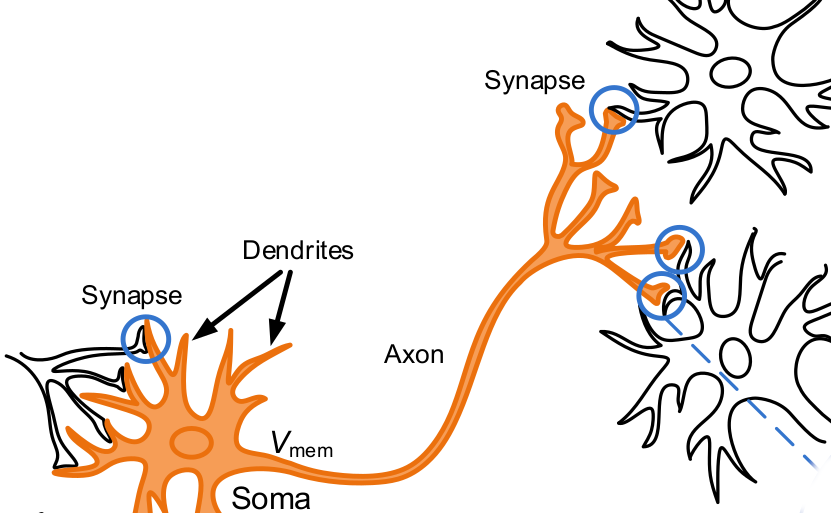
\includegraphics[scale=0.21]{neuron.png}
%\caption{Simplified diagram of a typical biological neural cell \cite{wu2015cmos}.}
%\label{bneuron}
%\end{wrapfigure}
Neuromorphic systems  include a large number of neurons, synapses and their interconnecting structure on hardware.  Such systems are highly parallel, fast, fault tolerant,  intelligent and
compact.  This research focus is on neuromorphic systems implementing Spiking Neural Networks (SNNs). 
Spiking neural networks  are the third generation of neural networks where neurons communicate through sparse sequences of spikes. Comparing to previous generations, SNNs
are faster, smaller in size, more energy efficient and biologically realistic [1,2]. 

 Implementation of SNNs is computationally expensive because of
nonlinear expressions in neuron models, size of the networks
and various communication pathways.
% A simplified  biological neuron with its corresponding connections is shown in Fig. \ref{bneuron}. A neuron could be connected to hundreds of the  other cells including neurons and astrocytes.    
 This research objective is to address this challenges by designing efficient and high speed hardware implementation platform for SNN.
\\ [0.2cm]
{\bf Methods: }
%
%One approach to study   biological neural networks is to divide it into two
%hierarchical sub-levels of components and architecture. The
%components level, representing the lowest level of abstraction,
%involves studying and mathematically modeling the properties
%and interactions of cells within the network. The architectural level,
%however, deals with the complex interactional behaviors of
%a large number of inter-connected components. Activities that
%occur at the architectural level include learning and 
%information processing in the biological neural networks. 
%
%At the cell level, this research has two objectives; First, is analyzing the cells  differential equation and performing bifurcation analysis  to  optimize these  ODEs for a high-performance and low-cost    implementation. Second, is designing efficient circuits for hardware implementation of these cells. These two objectives are clarified further in the following.
%
%
Current neuromorphic research has led to the development of a plethora of models to mimic real neurons with different levels of abstraction in biological details [3,4]. 
%Biologically-plausible models such as Hodgkin Huxley \cite{hodgkin1952quantitative}
%describe cellular phenomena and properties of the individual
%biological components. Such low-level models impose more
%computation cost, making it difficult to simulate large-scale
%networks. On the other hand, biologically-inspired models
%such as Izhikevich \cite{izhikevich2003simple}, aim to
%mimic the biological neurons to the best degree of accuracy.
%Such models can reproduce most of the firing patterns of real
%neurons and are easier to couple to other spike-oriented units.
%Moreover, high-level Integrate and Fire (IF) \cite{gerstner2002spiking} is another
%computationally efficient neuron model, but it cannot exhibit
%many essential features of the biological neurons as observed
%in experiments. 
The choice of models depends
on the application of the device to be designed. 
%To perform
%computations with SNNs only a simple IF or Exponential
%IF (EIF) may be enough to act as a thresholding box.
%However, for research in neuroscience, biologically plausible
%models have higher flexibility in mimicking biology.
 In this research we intend to focus on
biologically plausible and detailed models and optimize them without comprising their  correctness.  

 %Second objective at cell level is designing practical circuits realizing these cells using hardware implementation techniques (e.g.
  First objective at the lowest  level is designing practical circuits realizing brain cells using hardware implementation techniques (e.g. pipelining and power optimization techniques).  It is very important to implement the cell
models as efficient and fast as possible since they are basic building block of the neuromorphic systems. 
Biologically plausible models are  relatively complex in nature comparing to high-level models due to their large array of differential equations and accompanying parameters.
As a result, they have  seen limited
proposed hardware implementations. Currently, there is no neuromorphic processor available for large scale simulation of the biologically detailed models. 
 However these models are gaining
more attention by researchers. 


At the architectural and software levels, brain cells are connected together through different interaction mechanisms and their systematic behavior is analyzed. 
%T
%his is useful to study biological functions and disorders as well as discovering computational algorithms underlying information processing, learning and memory in the brain. 
This research has two objectives in architectural level; First is applying brain inspired learning and information processing algorithms in the software level and second is  designing a configurable hardware for large scale implementation of biological neural network. \\
%In the following,  I will explain these two objectives in more details. 
%
%
%
%The exact mechanism of information processing and learning algorithm in the brain is yet unknown. However, 
%Spike Timing Dependent Plasticity (STDP) is the most popular method  for unsupervised online training of 
%feed-forward  biological neural networks. This method is based on Hebbian learning where analogous to biology, the synaptic weight changes when a pre-synaptic neuron fires
%in a short time before or after the post-synaptic neuron,
%strengthening or weakening the neuron connection accordingly. Such a change is determined as an exponential of the time difference between two events. 
%
%Large scale hardware implementation of biological neural networks could be divided into two steps. First steps is implement nonlinear bio-chemical reactions between components and second  is to design an architecture to implement  various communication pathways. 
%\\ [0.2cm]
{\bf Previous Research: } 
My M.Sc. dissertation titled ``Digital Implementation of a Concise Model for Astrocyte Calcium Oscillations" was beginning of my research in the field of neuromorphic engineering where I optimized a biological astrocyte for hardware implementation using Piece Wise Linear (PWL) approximation technique. Since, I continued to research in spiking neural network and neuromorphic engineering. As a PhD student, I started using COordinate Rotation DIgital Computer (CORDIC) method to implement Izhikevch neuron and on-hardware online spike time dependent plasticity.  The advantage of CORDIC algorithm over previous methods including PWL, is its very high precision to calculate nonlinear terms and yet it is well suited for hardware implementation.  
%In another work, a  digital implementation of a biologically plausible astrocyte and glutamate-release mechanism was presented.  
% The designed hardware was capable of calculating nonlinear functions with a very
%high precision while having relatively high performance. This is most important because, unlike high level models, simulation of biologically plausible models 
%due to high biological details requires long time and computational
%power and will fall behind the real time easily. This hardware is
%most useful to emulate the tripartite synapse and its components.
The primary goal of those researches was to find an appropriate hardware for neurons, astrocytes and other biological cells as buildings blocks of a biological detailed neuromorphic processor.\\
{\bf Future Research }\\
My future research plan involves
 both studying  algorithms underlying learning and information processing in biological neural network as well 
 designing neuromorphic processor for large scale implementation of such networks. 
% Towards this objectives, I defined 4 projects. \\ [0.2cm]
%{\bf Project 1} 
%
%This project aims  to study the different models presented by researchers to mimic biological cells that are involved in information processing in the brain. The objective is to adapt and modify differential equation describing these models to maximize performance and minimize power consumption and area. Students will run computer simulation of these models and perform bifurcation analysis to look for possible modification or approximation in these models.
%\\ [0.2cm]
%{\bf Project 2} 
%
%Designing digital circuits for ODEs describing cells. Students will use hardware implementation and optimization techniques to increase performance and reduce power consumption and area of  designs. The circuits need to be simulated to ensure their validity. 
%\\  [0.2cm]
%{\bf Project 3} 
%
%Studying interactions of the cells within the biological neural networks and investigate the mechanisms behind  learning, information processing and 
%energy efficiency. Students will run computer simulations to observe changing of biological parameters and ions concentrations inside and around the cells that are active in learning and information processing.   
%\\  [0.2cm]
%{\bf Project 4} 
%
%Large scale implementation of the biological cells and   communication pathways in the biology. Students will design a new architecture capable of online on-chip learning with  biological neural networks. \\[0.2cm]
%%-------------------
%{\bf Research Program Feasibility} 
%
%\begin{wrapfigure}{l}{0.5\textwidth}
%\centering
%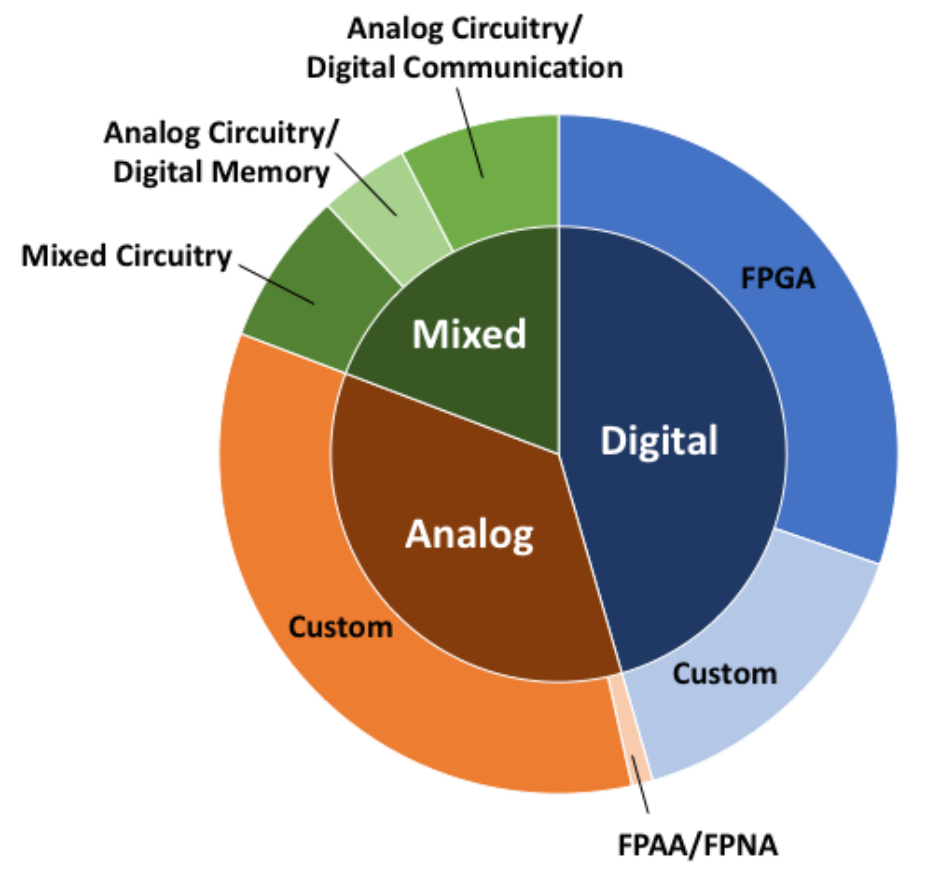
\includegraphics[scale=0.18]{hardware.png}
%\caption{An overview of hardware implementations in neuromorphic computing \cite{schuman2017survey}.}
%\label{fpga}
%\end{wrapfigure}
%The research would be initially computational, it can be  performed at a small
%undergraduate institution. 
Design prototypes would be implemented and tested on Field Programmable Gate Arrays (FPGAs) at first phase. FPGAs provide relatively cheap, fast, reconfigurable, and easy to work with platform for testing functionality and performance of the digital hardwares and are a popular implementation platform
 %as shown in Fig. \ref{fpga}.
  Second phase is designing an Application Specified Integrated Circuit (ASIC)  to implement the neuromorphic processor which require softwares such Cadence that currently are accessible   through CMC Microelectronics for universities. Finally, the design need to be fabricated that is also is supported by CMC Microelectronics.
  The primary goal of those researches was to find an appropriate hardware for neurons, astrocytes and other biological cells as buildings blocks of a biological detailed neuromorphic processor.\\
{\bf Future Research  }\\
My future research plan involves both studying  algorithms underlying learning and information processing in biological neural network as well designing neuromorphic processor for large scale implementation of such networks. Towards these objectives, I defined 4 projects. \\ 
{ Project 1:} 
This project aims  to study the different models presented by researchers . The objective is to adapt and modify differential equation describing these models to maximize performance and minimize power consumption and area. Students will run computer simulation of these models.
{ Project 2:} Designing digital circuits for ODEs describing cells. Students will use hardware implementation and optimization techniques to increase performance and reduce power consumption and area of  designs. 
{ Project 3:} 
Students will run computer simulations to observe changing of biological parameters and ions concentrations inside and around the cells that are active in learning and information processing.   
{ Project 4:} 
Large scale implementation of the biological cells and   communication pathways in the biology. Students will design a new architecture capable of online on-chip learning with  biological neural networks. 
{ Project 5:} software design and optimization for the hardware.
  \\
\hspace*{-1em}
{\bf References} \\
%\vspace*{-4em}
{\footnotesize
\phantom \quad [1] K. E. Friedl, A. R. Voelker, A. Peer, and C. Eliasmith, “Human-inspired neurorobotic system for classifying surface textures
by touch,” IEEE Robotics and Automation Letters, vol. 1, no. 1, pp. 516–523, 2016.\\[-0.1em]
\phantom \quad [2] F. Ponulak and A. Kasinski, "Introduction to spiking neural networks: Information processing, learning and applications.,"
Acta neurobiologiae experimentalis, vol. 71, no. 4, pp. 409-433, 2011.\\[-0.1em]
\phantom \quad [3] M. Samie, G. Dragffy, A. M. Tyrrell, T. Pipe, and P. Bremner, “Novel bio-inspired approach for fault-tolerant vlsi systems,”
IEEE Transactions on Very Large Scale Integration (VLSI) Systems, vol. 21, no. 10, pp. 1878–1891, 2013.\\[-0.1em]
\phantom \quad [4] A. L. Hodgkin and A. F. Huxley, “A quantitative description of membrane current and its application to conduction and
excitation in nerve,” The Journal of physiology, vol. 117, no. 4, p. 500, 1952.\\[-0.1em]
\phantom \quad [5] E. M. Izhikevich, “Simple model of spiking neurons,” IEEE Transactions on neural networks, vol. 14, no. 6, pp. 1569–1572,
2003.
}
%\newpage
 \thispagestyle{empty}
 %\lhead{Research statement}
 \phantom \quad \\
{\bf Case II: 
Post Quantum Hardware Cryptography and Homomorphic  Encryption}\\
%\vspace*{3\baselineskip}\\
This research program involves reducing complexity and efficient hardware implementation of the post quantum cryptography, homomorphic encryption, and homomorphic data processing embedded systems. \\[0.2cm]
{\bf Background:  } 
Cryptography systems have become  inseparable parts of almost every communication device.
Cryptography is  used to provide confidentiality, data security, and authentication in many applications such as
communication devices, autonomous vehicles, Internet of Things (IoT), healthcare [1,2,3,4] etc.


However, with rise of the quantum computers capable of executing Shor algorithm  [5], many popular public key cryptography systems including RSA  and elliptic curve cryptography will be no longer secure.  This would greatly endanger the security of digital communications and expose user's data. 
 National Institute of Standards and Technology (NIST) has already started a competition for developing cryptographic systems that are resistant to quantum computers attacks. At present, NIST has called for submissions for round 3 of this completion [6]. 
%The submission for previous rounds could be find in references \citecrypto{nistr2,nistr1}. 


Another issue with expansion of the Internet and cloud systems is privacy concern. 
 Currently, with the most secure communication between user computer and cloud system, still the data is decrypted in the cloud for processing. Therefore, the third parties owning the cloud and those with authorized access can read the data and use it for their own advantages. Homomorphic Encryption (HE), first introduced by Gentry  is a privacy preserving algorithm that allows valid computing over encrypted data without the need to decrypting it. 
 
 Since these algorithms are expected to be the future  cryptography systems, it is important to design an efficient  embedded systems for these systems. In next section,
 I further explain my methods to address this challenge. \\
{\bf Method: } 
Since  post quantum cryptography is a rather new field and because of  complexity of its algorithms, there exists only a limited number of the hardware implementations for these algorithms. 
 In this research proposal, Field Programmable Gate Arrays is selected as the initial implementation target since they provide a  reconfigurable, cheap and yet fast hardware platform. 
 % Round 3  finalists for public-key encryption, key establishment and digital signature are already available in NIST website. Most of these algorithms come only with a software implementation. Even those with hardware implementation still have plenty of room for improvement. This also applies to homomorphic encryption and computation as I discuss it further in the following. 
  In homomorphic encryption, plaintext is transformed into ciphertext, allowing computation on the encrypted data resulting in another ciphertext. Decryption of this ciphertext yields the same computation result as if it had been performed on plaintext.
 % \begin{figure}
% \centering
%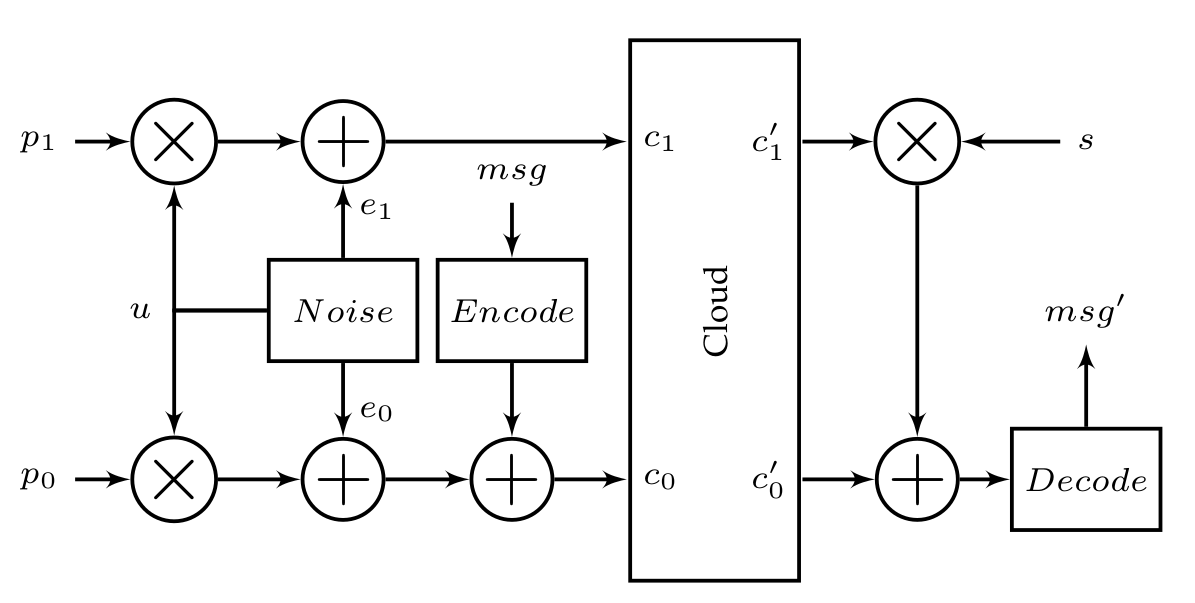
\includegraphics[scale=0.18]{fv.png}
%  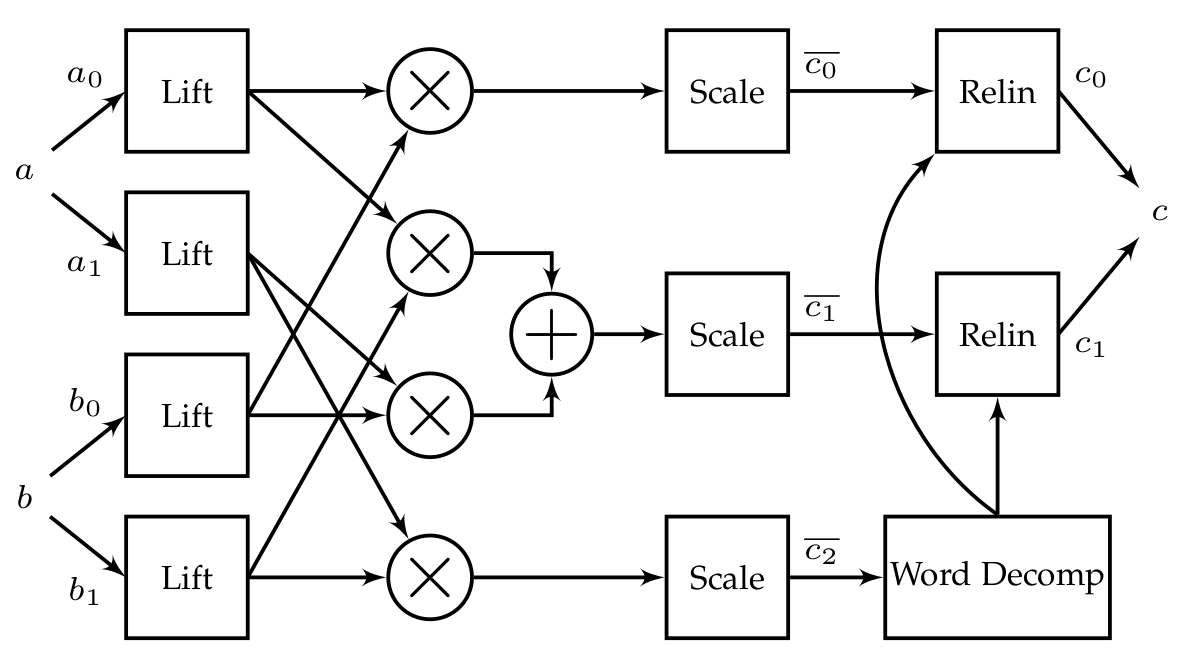
\includegraphics[scale=0.18]{fvhom.png}\\[-0.5em]
%(a)\hspace{7.2cm}(b)
%  \caption{(a) Fan and Vercauteren  (FV) encryption  encrypts a message into pair of ciphertexts c0 and c1 using public keys p0 and p1. 
%  (b) Fan and Vercauteren homomorphic multiplication over the ciphertexts (figures are taken from \cite{turan2020heaws}.)}
%  \label{hom}
% \end{figure}
% HE is based on lattice problems and adds noise during encryption. The value of this noise becomes greater each time an operation is performed on the ciphertext. 
% Somewhat Homomorphic  Encryption (SHE) scheme only allows limited number of the operations on the ciphertext and more than that, the signal to noise ratio becomes so large that the original data could not be recovered anymore. Gentry in his paper introduced use of bootstrapping technique which is basically homomorphic evaluation of
%the decryption circuit in the cloud to refresh and remove extra noises.
% This resulted into Fully Homomorphic  Encryption (FHE). 
 However, such  operations are computationally expensive and increases the complexity of the homomorphic  computations circuit. 
% Fig. \ref{hom} shows the circuit for homomorphic  encryption and homomorphic multiplication over encrypted data for  FV \citecrypto{fv} scheme. 
 Compared to software implementations, hardware cryptography results in a higher speed and a lower cost, while satisfying efficiency and low-power requirements of electronic
devices. Implementation of homomorphic encryption and evaluation circuit is a extremely challenging because of the very large word length of ciphertexts and computational unit, specifically multipliers. Homomorphic encryption  is a rather new research topic and its hardware implementation is less explored. In the following, I discuss my approach towards this  problem to achieve a better hardware for practical homomorphic encryption and data processing. 
%First, is studying the homomorphic encryption and computation to reduce their complexity and optimize them for hardware implementation. For instance, polynomial multiplication is 
%one of  the operations that is frequently performed over very large size operands (eg. 4096 coefficients of 180-bit size  ) and plays a key role in overall performance and cost of the hardware. Therefore, it is  important to optimize these algorithm as much as possible before implementing on hardware. 
%Second, is designing and efficient hardware architecture to encrypt and process data homomorphically. \\[0.2cm]
\\{\bf Previous Research: }
As postdoctoral fellow, I was working on the efficient  FPGA implementation of  finite field multipliers for Elliptic Curve Cryptography (ECC)  where we proposed a new binary polynomial multiplication algorithm with low complexity and high speed.
The work was then extended to to hardware implementation of lattice based cryptography  algorithms and other post-quantum encryption algorithms.
\\
% Currently, I am closely monitoring PhD students researching in post quantum cryptography and homomorphic encryption where their research is focused on designing an FPGA based embedded processor for these algorithms.  \\
{\bf Future Research (Research Plan): }
My future research plan engages both studying and optimizing post quantum and homomorphic  encryption  and computation algorithms as well as designing an efficient embedded processor and processor for these algorithms. 
%Towards this objectives, I defined 3 projects.\\[0.2cm]
%{\bf Project 1}
%
%This project aims to study the different algorithms presented by researchers for 
%post quantum cryptography including finalists of the NIST completion to standardize  quantum resistant public key cryptographic algorithms. The objective of this study is to reduce complexity and optimize these algorithms for FPGA implementation. 
%\\[0.2cm]
%{\bf Project 2}
%
%Investigating homomorphic encryption and ciphertext computation algorithms. Students will 
%perform mathematical analysis to enhance these algorithm in the terms of area and delay complexity. Further, they will run computer simulations to check validity of the algorithms. 
%\\[0.2cm]
%{\bf Project 3}
%
%Students will design an architecture and circuit to efficiently implement  these algorithms on hardware, either as accelerator for computer software or possibly as an standalone hardware cryptography system.\\[0.2cm]
\\{\bf Research Program Feasibility: }
For the first phase which is optimizing  algorithms for hardware implementation, I will use Python programming language to run simulations and check the validity of  modified algorithms.  Further, I will use FPGAs as implementation platform to measure efficiency of design. FPGAs are substantially cheaper than designing  and fabricating a VLSI ASIC and have advantage of flexibility. Eventually, after testing design could be fabricated for final evaluations. Towards this objectives, I defined 3 projects:
 Project 1: 
This project aims to study the different algorithms presented by researchers for 
post quantum cryptography including finalists of the NIST completion to standardize  quantum resistant public key cryptographic algorithms. The objective of this study is to reduce complexity and optimize these algorithms for FPGA implementation. 
{ Project 2:}
Investigating homomorphic encryption and ciphertext computation algorithms. Students will 
perform mathematical analysis to enhance these algorithm in the terms of area and delay complexity. Further, they will run computer simulations to check validity of the algorithms. 
{ Project 3:}
Students will design an architecture and circuit to efficiently implement  these algorithms on hardware, either as accelerator for computer software or possibly as an standalone hardware cryptography system.
\\{\bf Funding for research }
In terms of funding , I would be able to use my background and familiarity with problems and concerns of industry to secure funding for the research. I have also experience of writing successful research proposal with industry partner to obtain MITACS grant. \\ 
\hspace*{-1.8em}
{\bf References} \\
%\vspace*{-4em}
{\footnotesize
\phantom \quad [1] J. Yoo and J. H. Yi, “Code-based authentication scheme for lightweight integrity checking of smart vehicles,” IEEE Access,
vol. 6, pp. 46731–46741, 2018.\\[-0.1em]
\phantom \quad [2] R. Abu-Salma, M. A. Sasse, J. Bonneau, A. Danilova, A. Naiakshina, and M. Smith, “Obstacles to the adoption of secure
communication tools,” in 2017 IEEE Symposium on Security and Privacy (SP), pp. 137–153, 2017.\\[-0.1em]
\phantom \quad [3] P. Aparna and P. V. V. Kishore, “Biometric-based efficient medical image watermarking in e-healthcare application,” IET
Image Processing, vol. 13, no. 3, pp. 421–428, 2019.\\[-0.1em]
\phantom \quad [4] T. D. P. Bai, K. M. Raj, and S. A. Rabara, “Elliptic curve cryptography based security framework for internet of things (iot)
enabled smart card,” in 2017 World Congress on Computing and Communication Technologies (WCCCT), pp. 43–46, 2017.\\[-0.1em]
\phantom \quad [5] P. W. Shor, "Algorithms for quantum computation: discrete logarithms and factoring," Proceedings 35th Annual Symposium on Foundations of Computer Science, 1994, pp. 124-134, doi: 10.1109/SFCS.1994.365700\\[-0.1em]
\phantom \quad [6] “Post-Quantum Cryptography-Round 3 Submissions,” 2020.

}
\newpage
 \thispagestyle{empty}
 \lhead{Teaching Statement}
 \phantom \quad \\
 {\bf Teaching Statement}
\vspace*{3\baselineskip}\\
{\bf Inspiration}

My father was a teacher. He always inspired me to learn by asking questions and intriguing my sense of curiosity. The same sense of curiosity  that grew my motivation to continue  my education and become a researcher. One quality that I most like about him and later, became a part of my character as well, was his critical way of thinking and teaching.  Instead of giving direct answers to my questions, he guided me and encouraged me to discover the answers for myself.
 From what I learned, it is the disciplined practice of critical thinking that
enables  students to examine ideas, determine their validity and become creative.  
In short,  a great teacher provides students with the motivation toward becoming a knowledgeable and innovative person.
My approach to teaching
 is based on same idea of critical thinking and has three main components: Inquiry,  a deep understanding, and novelty.
 \\ [0.2cm]
{\bf Inquiry }

I believe that the best way  to encourage students is inquiry-based learning. 
Students tendency toward a new concept will be higher when they believe that it can be answer to a problem in their minds.  
The idea is to start the class with a few well-chosen questions and have the students explore the topic themselves, with guidance from the teacher. 
In this method, I will express the fundamental problem,
 encourage my students with a desire to know the answer and then  let the class  discusses it. 
 My role would be more an moderator who leads students in a challenging experience  planned to promote discussion, thinking and discovery. As an example,  when I started Digital Logic Design at  beginning of the semester and intended to talk about number systems,  I initiated the class with the questions  "why predominant number system is decimal and why not for instance, octal or hexadecimal?"
 And after discussing that, I asked the next question "now, why machines use binary number system?".  I observed that larger number of students engaged in answering the second question, when the first question was discussed in advance, compared to classes when I went directly for the second questions. 

%As an example, I when I started Digital Logic Design at  beginning of the semester and intended to talk about number systems,  I initiated class with the question  "why the predominant number system is decimal and why not for instance, octal or hexadecimal?"
%I observed that these question intrigues students sense of curiosity.
% And after that I asked another question "why machines use binary number system?".
% I observed that number of  students  participate in the class  answering this question increase when the first question asked before this. 

 
 
 This method also leads to conceptual understanding of the the problems and solutions in electrical engineering.    
   Students with conceptual understanding know more than solitary facts and methods and are able to  connect different concepts, decipher problems,  and apply engineering methods in novel ways. \\[0.2cm]
   {\bf A Deep Understanding}
   
   A good teaching method is a combination of different  techniques. Another technique that I find to be most useful is  cognitive learning where learning focus is on understating the 
subject at the deeper level rather than memorization of approaches toward certain problems.
  My approach toward this process is based on the following elements:  First, students need to understand why they are learning the subject. Second, is gaining knowledge about the subject at a deep level and third, is to contemplate on the application of what they learned. 
 The course contents need to be designed in a way that the students get a deep understanding  and develop the skills to apply their knowledge in their field. 
    
    An example is when I was presenting logical operations (AND, OR and NOT) at a Digital Logic Design class. First, I explained the concept of idealized switches network 
    where switches are considered as having only two exclusive states of open or close. Further, I gave them simple examples and  asked them    to identify different combinations and make separate components.      Later, I  introduced the Boolean algebra and logical
operations as a way to analyze and design circuits by algebraic means in terms of logic gates. \\[0.2cm]
   {\bf Creativity}
   
Perhaps the most important part of learning  and at the highest level, is creativity. 
    The scientific approach toward creativity involves studying  and mastering what have been achieved so far, asking  questions, proposing  solutions, designing experiments to check validity of the solutions and finally communicating the research with other scientists to have feedbacks. 
    
    My plan to engage graduate  and last year undergraduate students in research would be by means of the following. First, I will give them enough background and knowledge in a specific area which I believe have potential for research. Further, I will ask them to identify and make a list of the new and prominent works published in the subject. Afterwards, I will ask them to write a short brief on those papers and identify  their contributions. The next step would be presentation of the papers that foster deeper understanding of the works. Personally, I believe explaining something to someone else helps to have better insight about the topic.  Therefore, such conferences would be an fundamental part of my approach which  helps students both to evaluate the literature and communicating their findings.    
    
    The next move would be critical analysis of the papers. Students need to think about the weaknesses, limitations and drawbacks of the proposed approaches. Performing simulations in order to   replicating and testing findings on the papers also helps them to 
    learn the required tools and approaches toward the problems and also facilitate spotting the problems.
    
    At end of any phase, it is my duty as a teacher to evaluate their work and give them feedbacks and suggestions to improve their work. This will give students the opportunity to improve their ability to identify the problem, review the literature  for solutions, propose new solutions and finally communicating their research. 
    
    
    In summary, I wish to give back those qualities that meant the most to me during my
education: inquiry, a deep understanding and creativity. I hope to develop the love of engineering in my students since personally, I feel an infinite passion for it. As a saying states: "Choose a career you love and you will never have to work a day in your life".

%\newpage
% \thispagestyle{empty}
% \lhead{Diversity Statement}
% \phantom \quad \\
% {\bf Diversity Statement}
%\vspace*{3\baselineskip}\\
%
%
%
%I was born in Iran,  in a city close to Iraq border, during the long and bloody war between Iran and Iraq. My parents had to leave everything behind and flee to  safer zones several  times. When I was three years old, there was a ceasefire and war was finally over after eight years. I don't remember much about the war; However, I could clearly feel and see the aftermath. There were people who lost their loved ones and were always sad, some lost a limb and became disabled, many suffered mental problems and most people, including our family, lost their home and all possessions because of bombings. This war, that left more than one million casualties and losses, was mainly over religious difference. I 
%deeply sensed and suffered from consequences of a flare up religious hate, and  as a child,  promised myself that never let hatred grow in my heart and I do everything I can to help people tolerate and understand each other. 
%
%
%Like many, we lost our home during aerial bombardments. My father was a teacher and we were fortunate to have a source of income.  Still, economy of the country was devastated after the war. My father  could only afford to build a room in ruins of our house and there was no electricity or running water.   Stealing and street violence crimes started to increase   in a way that my father  had to walk me to school before going to his work. 
% It was not uncommon for my neighborhood friends to have a drug abusing parent, a single parent household,  or experience domestic violence.   Living under such circumstances were   difficult but it gave me a valuable experience and I  can still fully understand  how it feels to be financially insecure and live in a dangerous neighborhood. 
%
%
%
%
%Later in school, I faced yet another challenge. Our city was a Kurdish region and I used to speak Kurdish with my family, friends and everyone else. However, the official language in the school and all textbooks were in Persian. Speaking Kurdish was forbidden in school and It was very difficult for me as child to suddenly start reading, writing and speaking a new language. I became fluent in the language, but moving out to other cities to continue education and subsequently finding a job where I faced more and more discrimination and
%humiliation because of my background. 
%
% As results of such systematic racism and being culturally oppressed, many people were ashamed to talk their mother tongue and begin to hide their ethnicity.  To fight this, I started a blog and developed android applications  to rise awareness that everyone has the right to speak their mother tongue and no body should ever be shamed of his race or background. My experience as a member of an
%ethnic minority has greatly helped me to better understand others who face similar
%challenges based on their identity.
%
%
%
%
%
%
%
%My commitment to promoting diversity and inclusion in academia is grounded in my personal experience. During my PhD in Canada, I was fortunate to work alongside insightful faculty members in University of Windsor. I was truly inspired by their commitment to social justice, diversity and inclusion. I became friends with people from  LGBTQ community.  Hearing their stories and experiences, and learning that some are still afraid to come out and be honest about their identity, reminded of my own experience as an ethnic minority. 
% I truly admired them and hope that one day no one experience stigma and discrimination because of sexual orientation. 
%  I have had the opportunity to address diversity and inclusion  in my roles as Graduate Assistant and Postdoctoral Fellow at University of Windsor. 
% I am committed to create an environment free from discrimination based on the race, religion, sex, economic status, sexual orientation, disability or other characteristics.
% 

\end{document}
